\documentclass[11pt]{article}
%\usepackage{CJK,CJKspace}
\usepackage{hyperref}
\usepackage{url}
\usepackage{amsthm,enumitem}
\usepackage{graphicx}
\usepackage{algorithmic}
\usepackage{geometry}
\usepackage{setspace}
\usepackage{indentfirst}
\usepackage{epsfig,tabularx,amssymb,amsmath,subfigure,multirow}
%\usepackage[margin=0.5in]{geometry}
%\input myfonts
\newtheorem{lemma}{Lemma}

\newtheorem*{claim}{Claim}
\renewcommand{\baselinestretch}{1.5}
\newcommand{\nop}[1]{}
\begin{document}

\newgeometry{left=1in,right=1in,top=1in,bottom=1in}
\centerline{\bf \LARGE Visualization of MovieLens Rating}
\bigskip
\centerline{\bf \LARGE Process Book}
\bigskip
\bigskip
\centerline{\bf \Large Zhao Chang u0931132@utah.edu u0931132}
\centerline{\bf \Large Junwei Shi u0943296@utah.edu u0943296}
\centerline{\bf \Large Tengda Shi tengda.shi@utah.edu u1015168}
\bigskip
\centerline{\bf \Large Project Repository: \url{https://github.com/VaultB0Y/dataviscourse-pr-visualization}}

\section{Overview and Motivation}

The objective of our project is to perform an interactive visualization analysis on the relationship between different kinds of movies and people who give ratings on the movies. Our project deals with a really interesting problem. Note that thousands of movies are released over the world each year. We can easily find the corresponding information in some online web sites (eg. IMDB\footnote{\url{http://www.imdb.com/}}). However, in fact, we are only interested in a small part of them. We have no time to scan all the introductions to these movies. Thus, we hope we can perform an interactive visualization analysis and tell people what movies they may like to see based on people's attribute information. These attribute information regarding different people can also be added into existing recommendation systems and improve the accuracy of recommendation.

\section{Related Work}

Existing works regarding recommendation systems inspire us to finish such a project. There are three major approaches used in prior works. The first one is collaborative filtering. It has been used in a lot of highly cited papers \cite{WWW2001,IEEE2003}. It does not rely on profile information of users and items. Also, it does not need any knowledge engineering effort. However, it requires some form of rating feedback. Also, it cannot solve cold start for new users and new items \cite{IJCAI2013}. The second one is content-based recommendation. It has already been used in some early works regarding recommendation algorithms \cite{AAAI1998,DL2000}. It only makes comparisons between items possible and does not require any community information. However, it needs some necessary content descriptions. Also, it cannot solve cold start for new users. The third one is knowledge-based recommendation. It is also used in a few research works \cite{ELIS2000,WWW2008}. It makes deterministic recommendations and ensures the quality of recommended items. Also, it can solve the cold start problem. However, it only works for static recommendations well and does not react to short-term trends. Recently, there are also some new approaches proposed by researchers. For example, some works improve traditional recommendation systems by adding social network analysis \cite{WWW20082,UCS2011}. Some works extract entities in users' tweets or weibos and add such information into existing frameworks for achieving advanced recommendation systems \cite{RS2009,IR2011}.

However, all these works focus on how to recommend products for users accurately. These recommendation algorithms are usually performed based on some complicated mathematical deductions. However, it seems difficult for such algorithms to explain how they can generate reasonable results \emph{in an intuitive way}. Therefore, we need to utilize the visualization tools. We perform an interactive visualization analysis and tell people what movies they may like to see based on people��s attribute information.

The visualization in this web site\footnote{\url{http://benfry.com/isometricblocks/}} inspires us to design Figure \ref{fig:fig12}. Figure \ref{fig:fig12} can easily reveal the dependencies of users with different attributes and different kinds of movies.

\section{Questions}

The primary questions we are trying to answer with our visualization are:
\begin{itemize}
\item Tell people which movie they may like to see. If you plan to watch a movie but you are not sure if you will like this movie, then you can see the ratings of people who are in your ages through our visualization and decide whether to go to see the movie.
\item For people in different ages, check what their favorite movies are and the ratings of each certain movie. The basic function of our visualization is to provide the services for users to search the information they want to check about the movies.
\item Help the movie makers to investigate who like their movies best. Our visualization will also benefit the movie makers and help them to make movies that more people like to watch.
\end{itemize}

What we would like to learn is if any trends or patterns exist in our data set. In particular, the things we would like to accomplish include:
\begin{itemize}
\item Show all the ratings of each movie, including the information of people who generate these ratings.
\item Show different ratings of different movies generated by each person. People can search the information according to the audience's gender, occupation, postal zone and so on.
\item Movies can be searched by category, theme, year and so on.
\end{itemize}

How do these questions evolve over the course of the project?

TBD

What new questions do you consider in the course of your analysis?

TBD

\section{Data}

We use MovieLens 1M Data Set\footnote{\url{http://datahub.io/dataset/movielens}}. This data set contains 1,000,209 ratings applied to 3,952 movies by 6,040 users of the online movie recommender service MovieLens. All ratings are contained in the file ``ratings.dat'' and are in the following format: UserID::MovieID::Rating::Timestamp. Ratings are made on a 5-star scale. Each user has at least 20 ratings. User information is in the file ``users.dat'' and is in the following format: UserID::Gender::Age::Occupation::Zip-code. Movie information is in the file ``movies.dat'' and is in the following format: MovieID::Title::Genres. By performing visualization analysis on the data set, we can answer some interesting questions, such as ``what kinds of movies are liked by people with some specific attributes''.

We pre-process the data set by clustering the data according to the different kinds of movies and different attributes of people. After generating such aggregation information, we use the transformed data set to perform interactive visualization analysis on it.

\section{Exploratory Data Analysis}

TBD

\section{Design Evolution}

\subsection{Our Design in Proposal}

In our design, we divide the whole framework into five parts:

\begin{itemize}
\item[1)] Present the rating information given a specific user.
\item[2)] Present the rating information given a specific movie.
\item[3)] Process the statistic given a specific user group using filtering.
\item[4)] Process the statistic given a specific movie group using filtering.
\item[5)] Find the dependencies of users with different attributes and different kinds of movies.
\end{itemize}

\subsubsection{Part 1 Design}
We can search the rating information given a specific user. Also we could filter out some types
of movies we do not need, such as released year and genres (as shown in Figure \ref{fig:fig1}). After that, we can present the
information grouped by genre, or just a scatter plot along the year x-axis. (see Figure \ref{fig:fig2} and \ref{fig:fig3}). Also
we can rank the movies as shown in Figure \ref{fig:fig11}.

\subsubsection{Part 2 Design}
We can search the rating information given a specific movie. We could present some interesting
statistics, such as number of ratings or scores, categorized by ages. (Figure \ref{fig:fig5} and \ref{fig:fig6}), or categorized
by some interesting features such as locations. Please note that Figure \ref{fig:fig6} is a distribution figure,
and we use different colors to denote the distribution percentage.

\subsubsection{Part 3 Design}
First we need to filter out the users we want, by selecting some features as in Figure \ref{fig:fig7}. Then we
show the statistics as Figure \ref{fig:fig5} and \ref{fig:fig6}.

\subsubsection{Part 4 Design}
We can filter out the movies by selecting features as shown in Figure \ref{fig:fig4}. We can show the statistics as shown in
Figure \ref{fig:fig9} and Figure \ref{fig:fig10}.

\subsubsection{Part 5 Design}
After some preprocessing of the data, such as clustering or collaborative filtering, we can show
the dependencies of different groups of users and the movies. The groups are based on the features
we have selected.

\begin{figure}[h]
\centering{
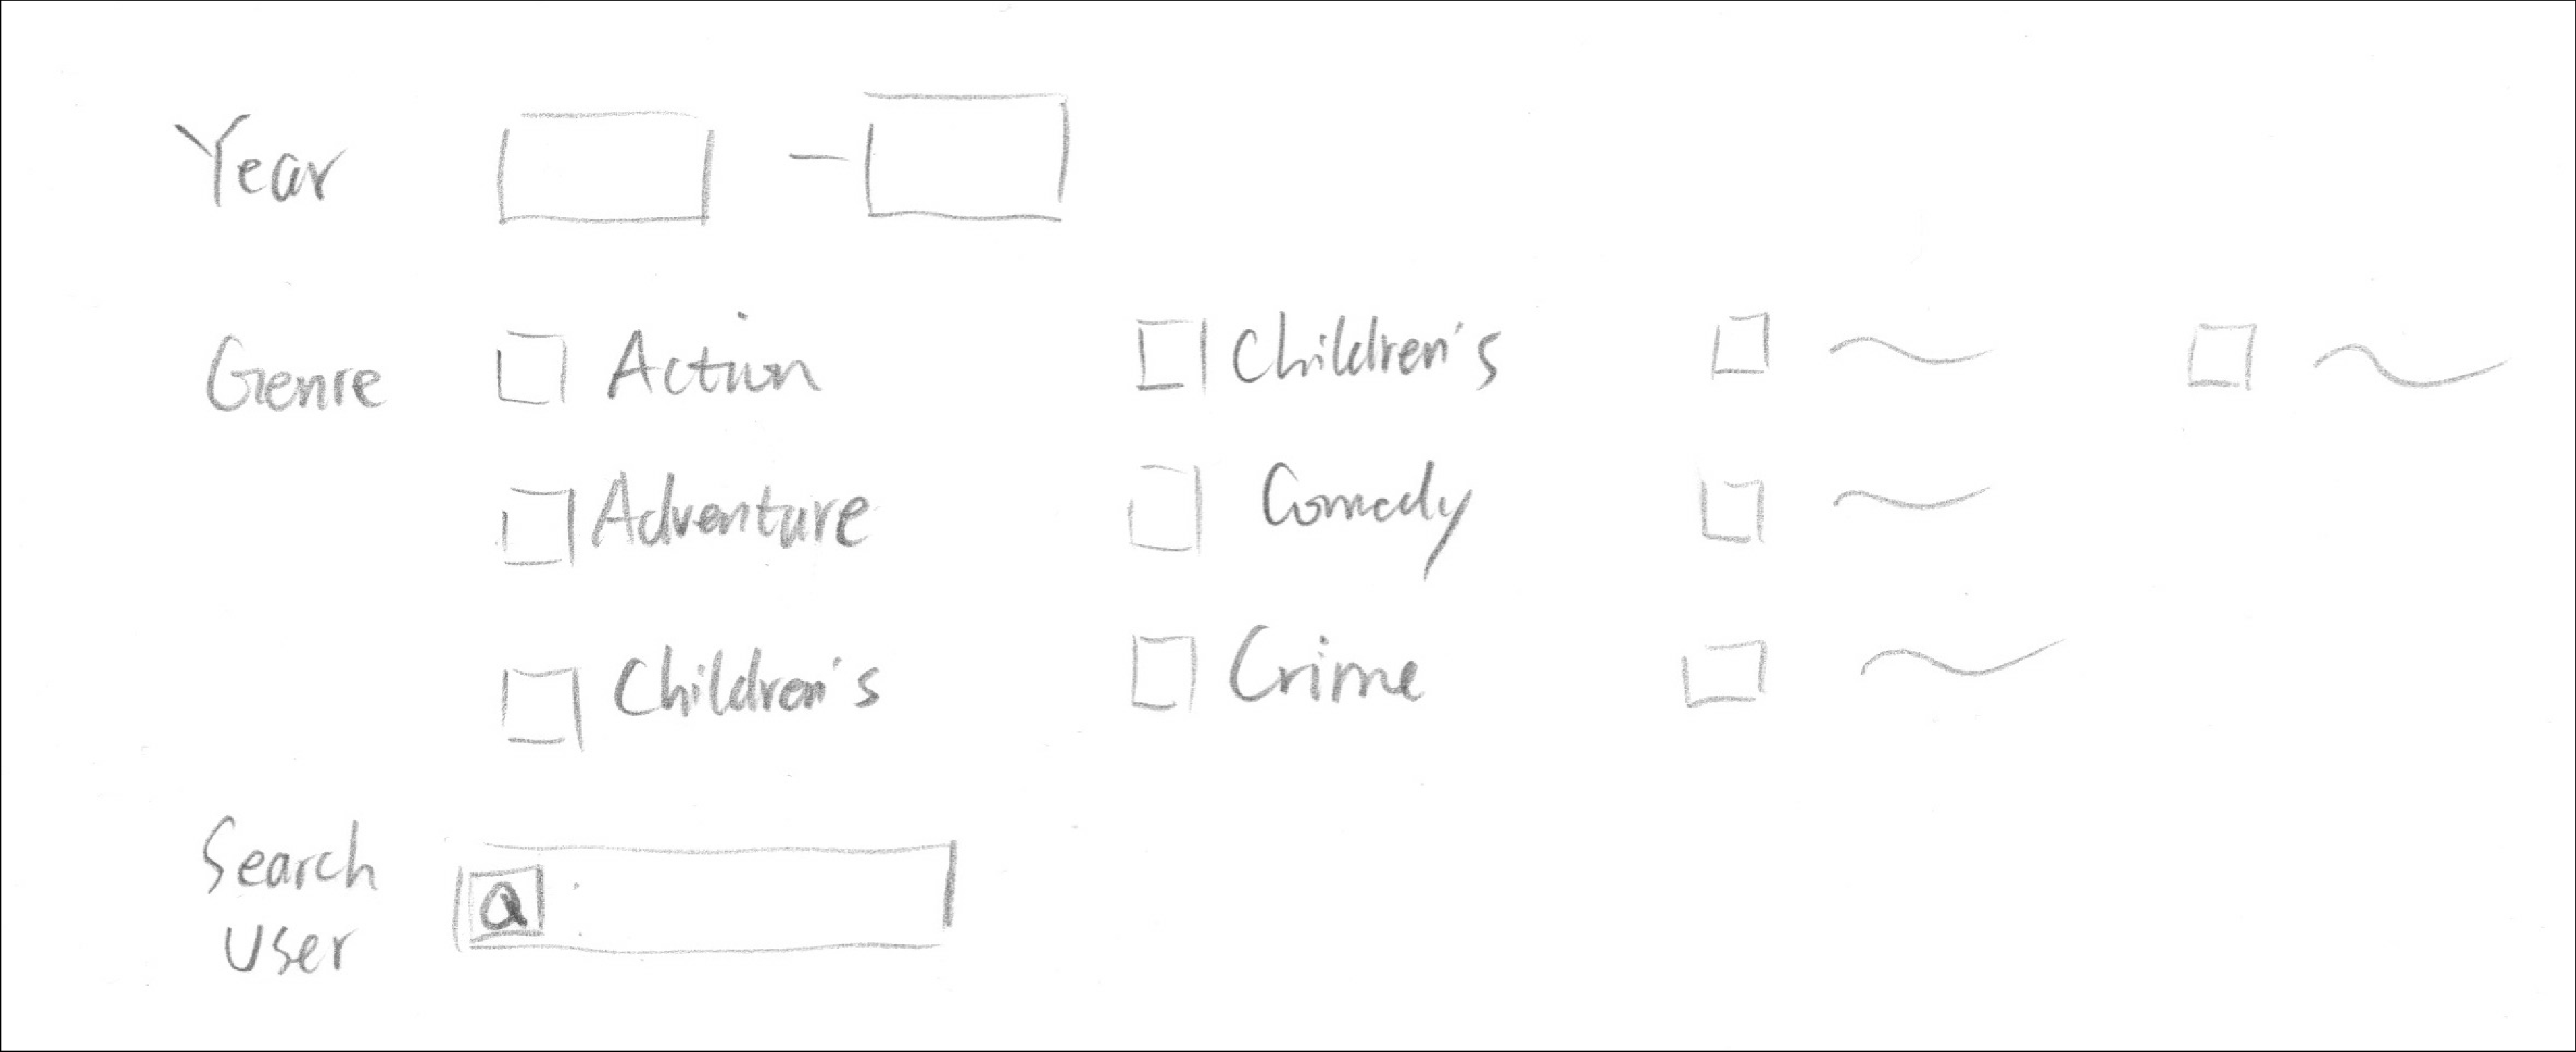
\includegraphics[width=.7\linewidth]{1.pdf}
}
\caption{Search for user and filter the movie information}
\label{fig:fig1}
\end{figure}

\begin{figure}[h]
\centering{
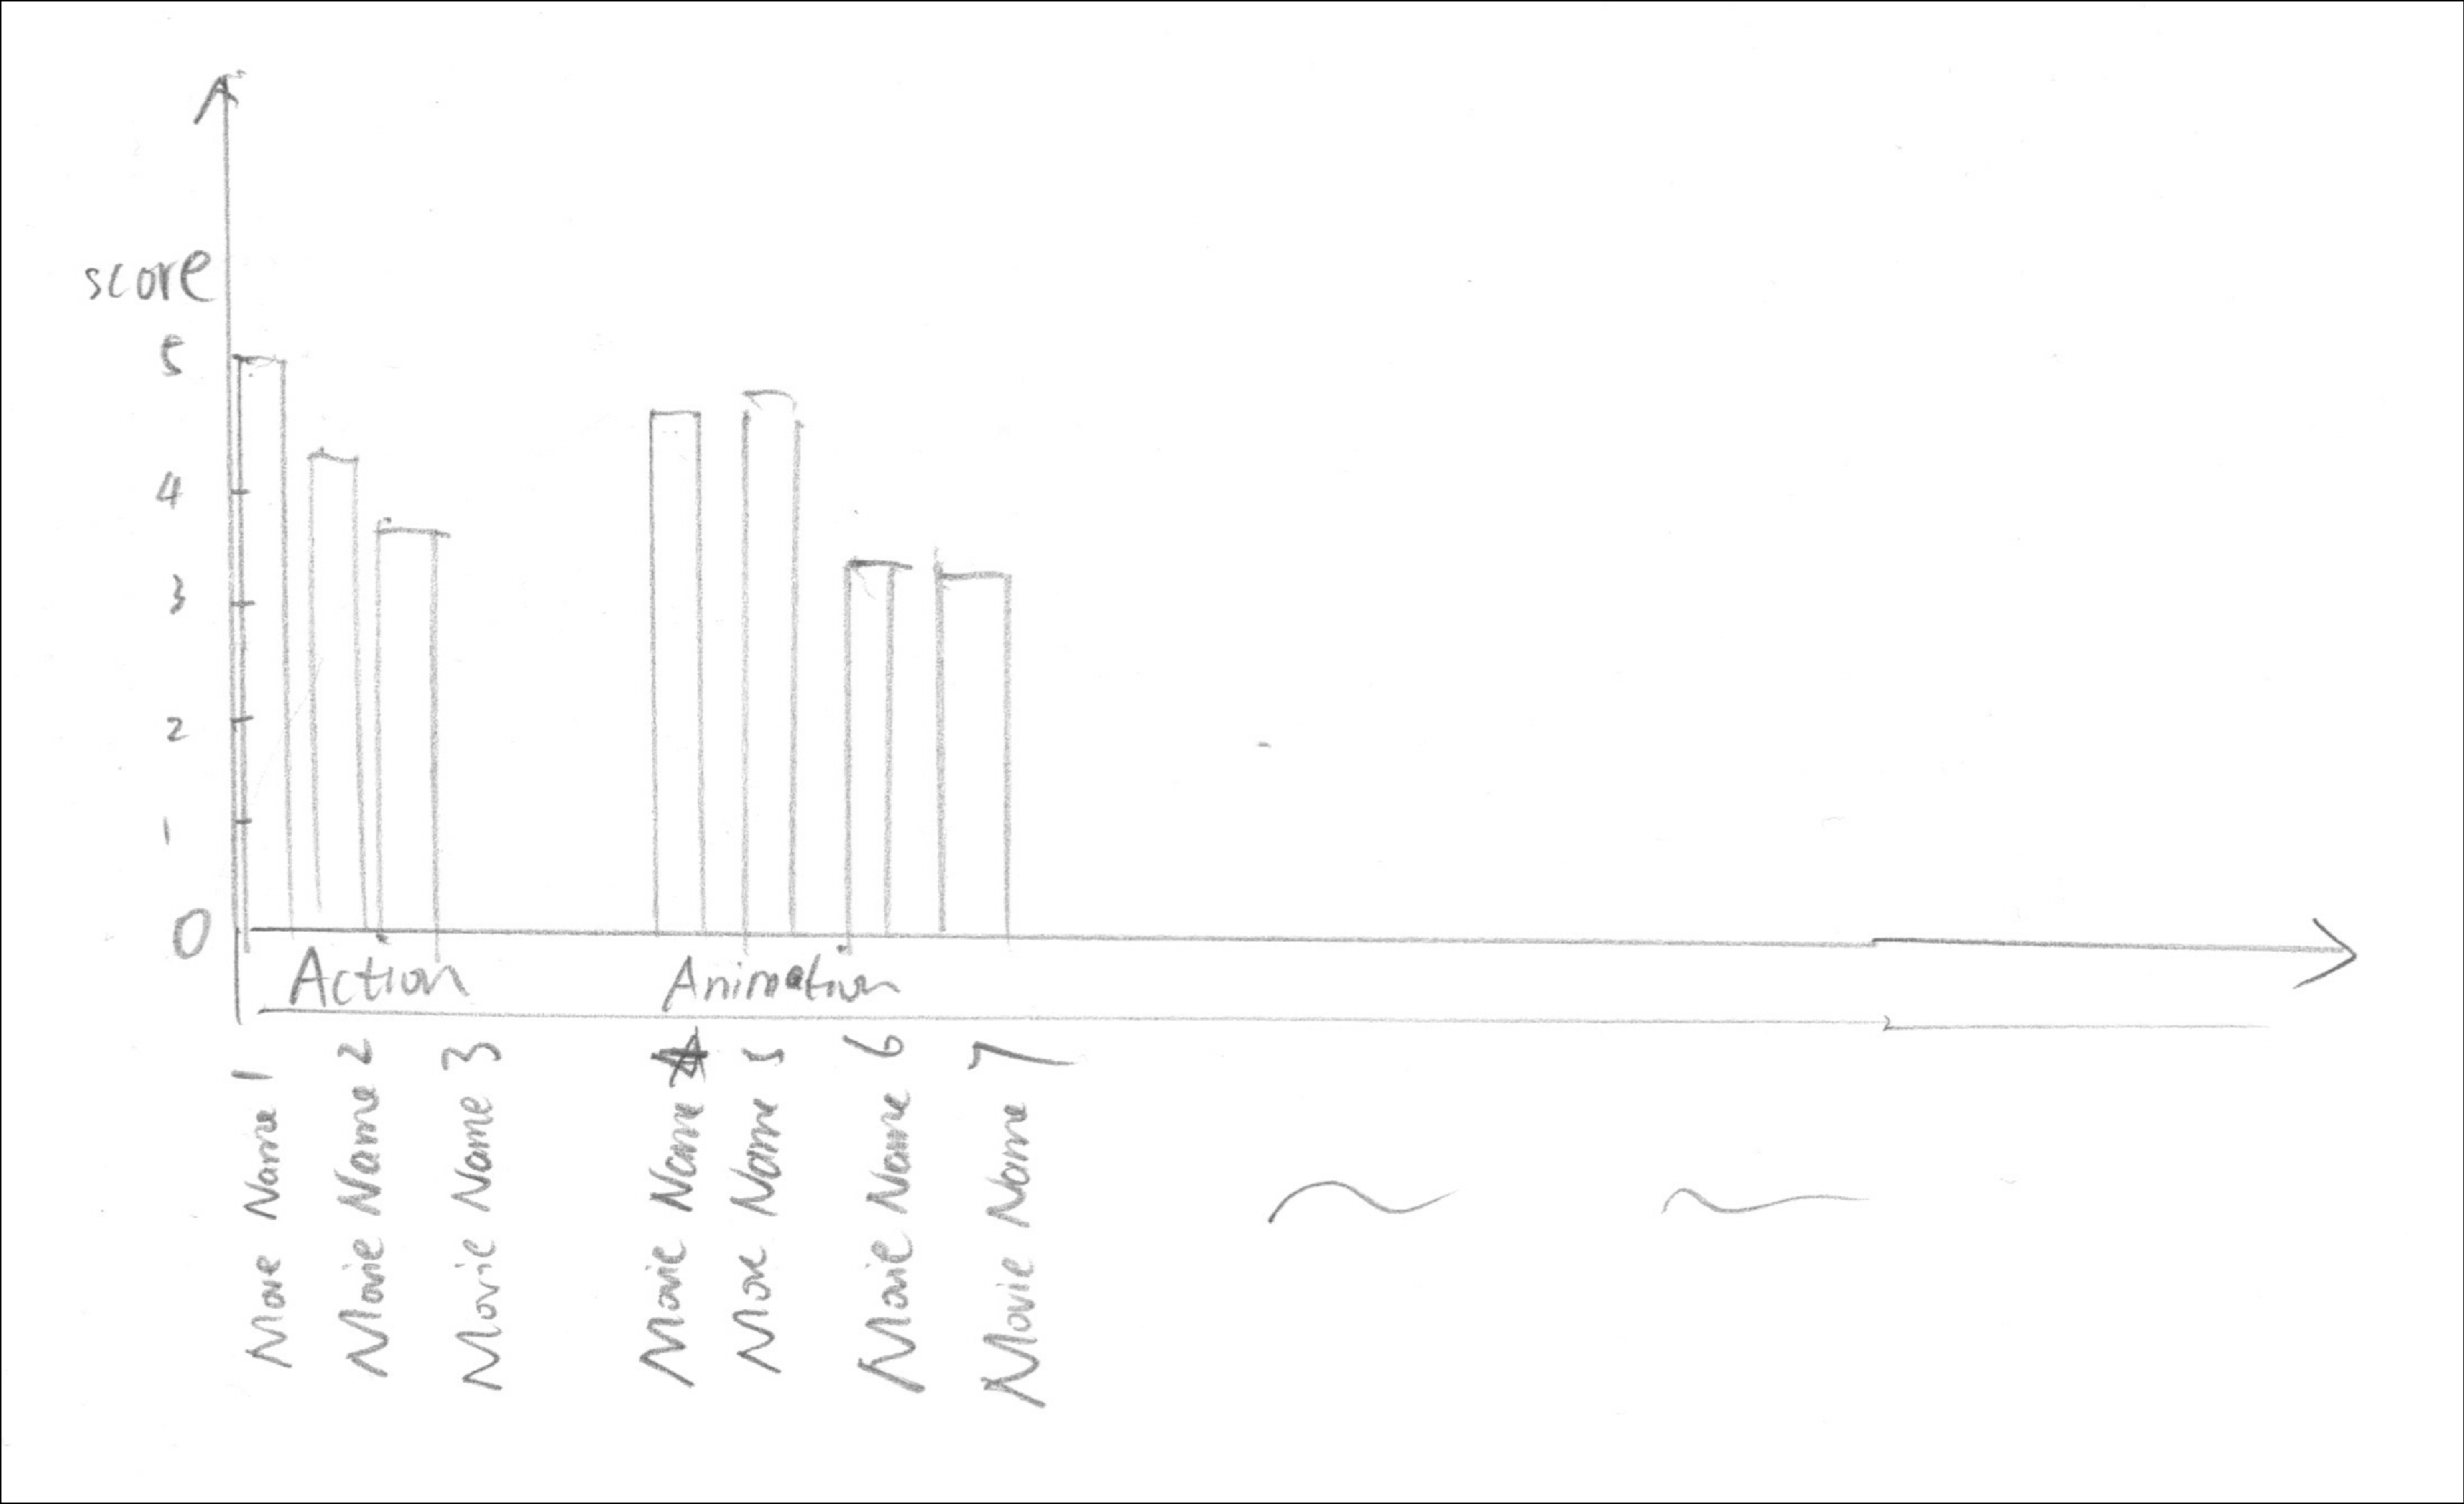
\includegraphics[width=.7\linewidth]{2.pdf}
}
\caption{Histogram of ratings grouped by genre}
\label{fig:fig2}
\end{figure}

\begin{figure}[h]
\centering{
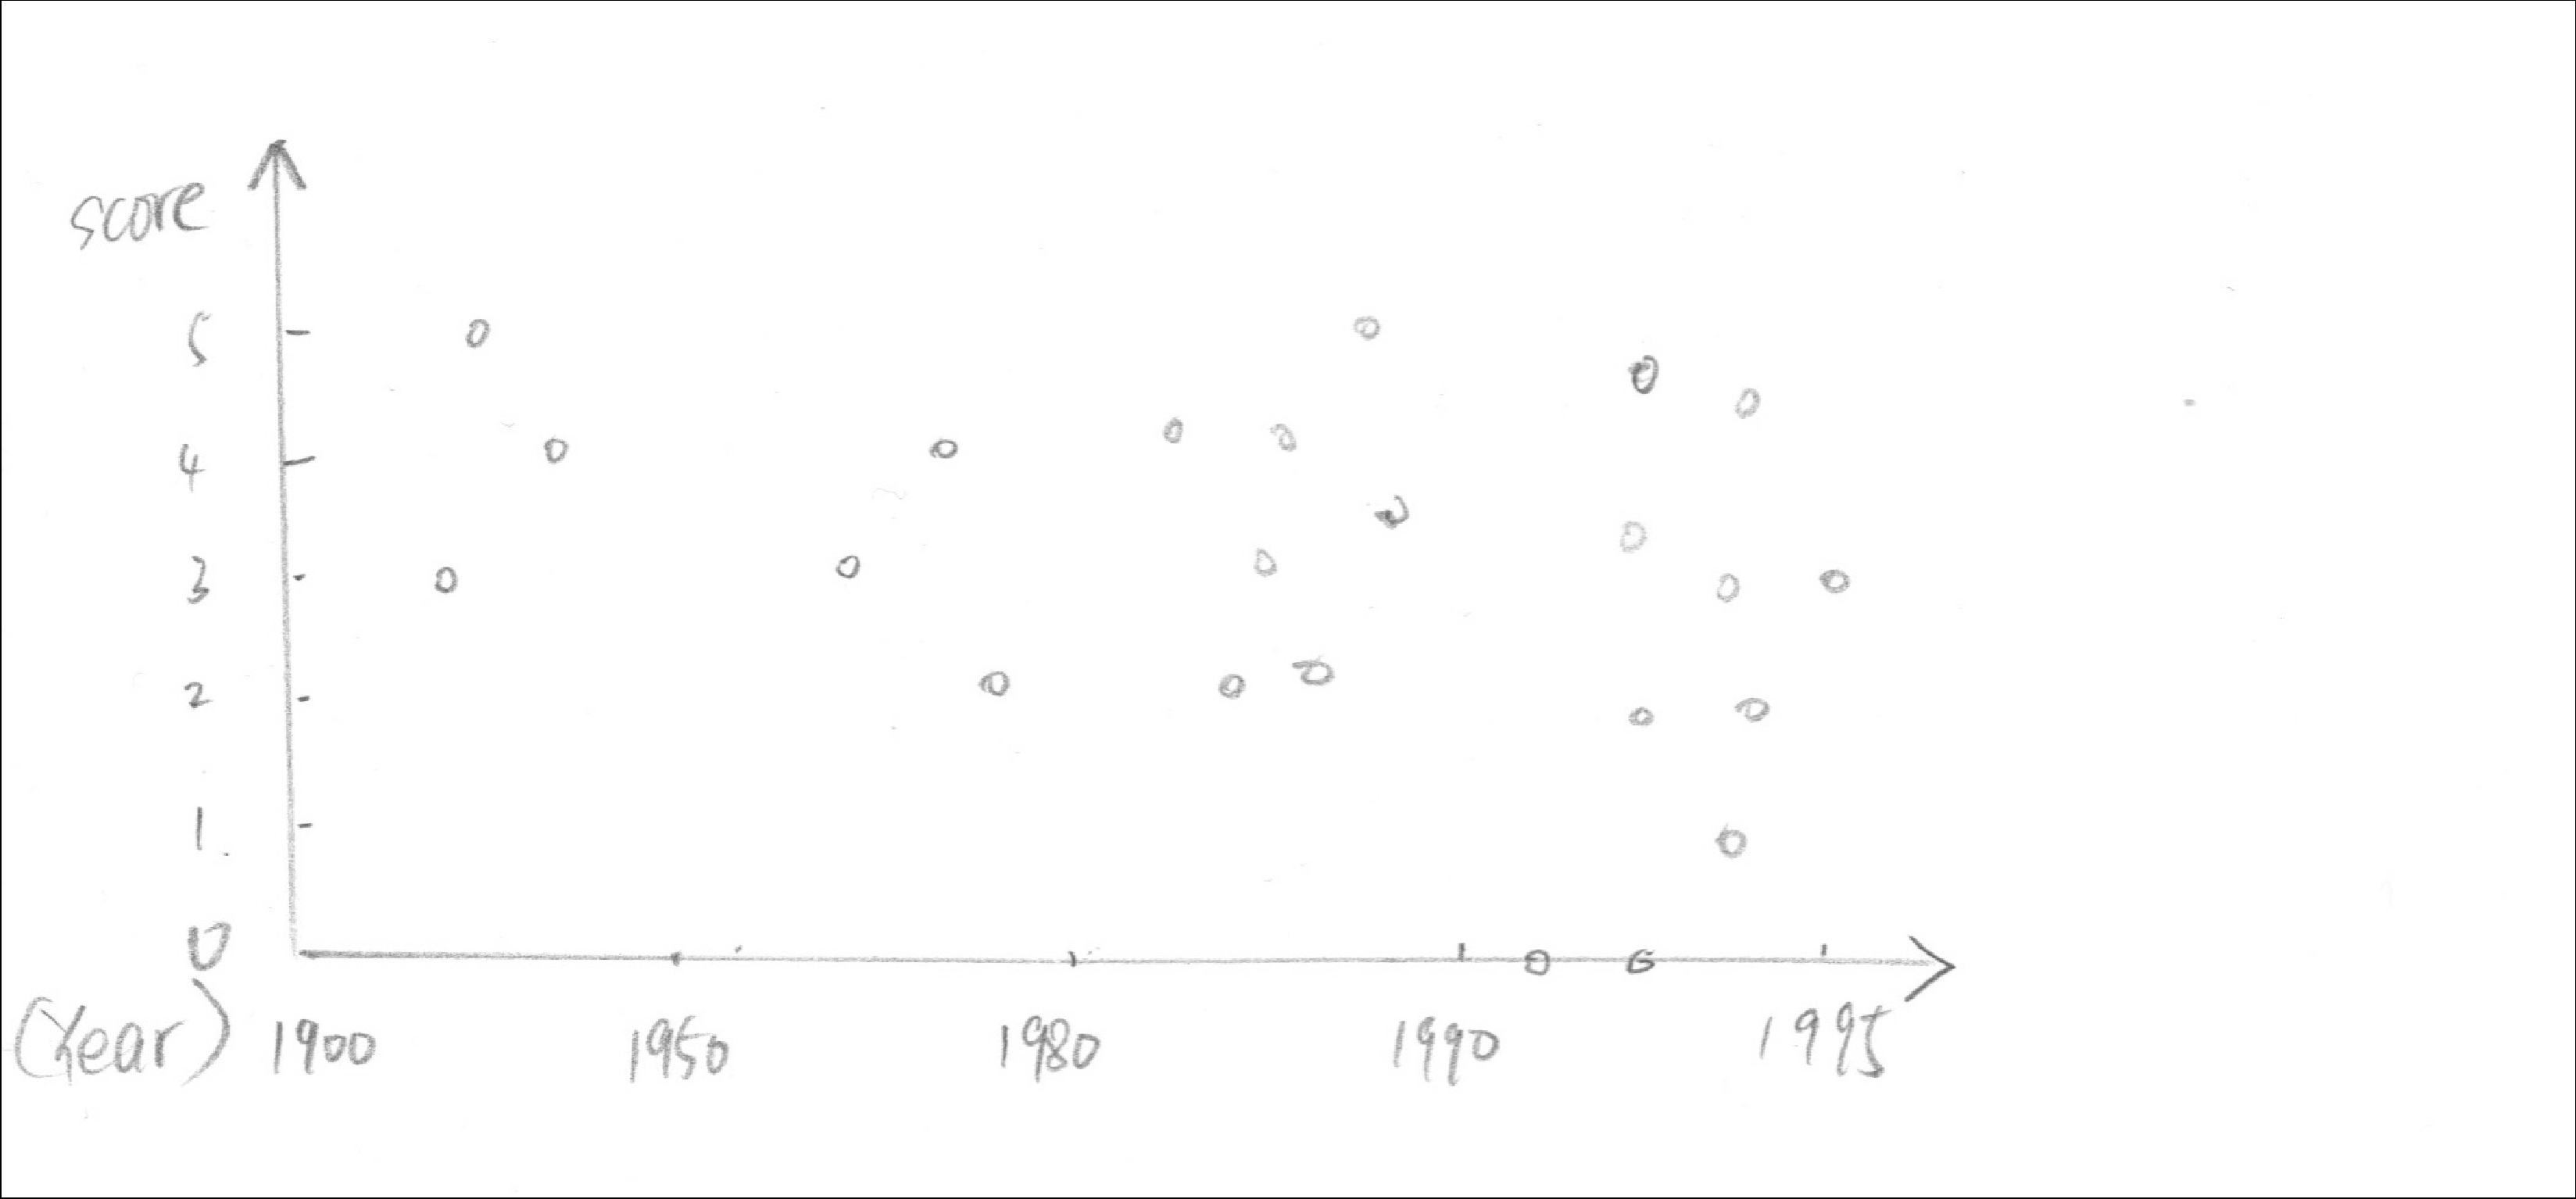
\includegraphics[width=.7\linewidth]{3.pdf}
}
\caption{Scatter plot of ratings}
\label{fig:fig3}
\end{figure}

\begin{figure}[h]
\centering{
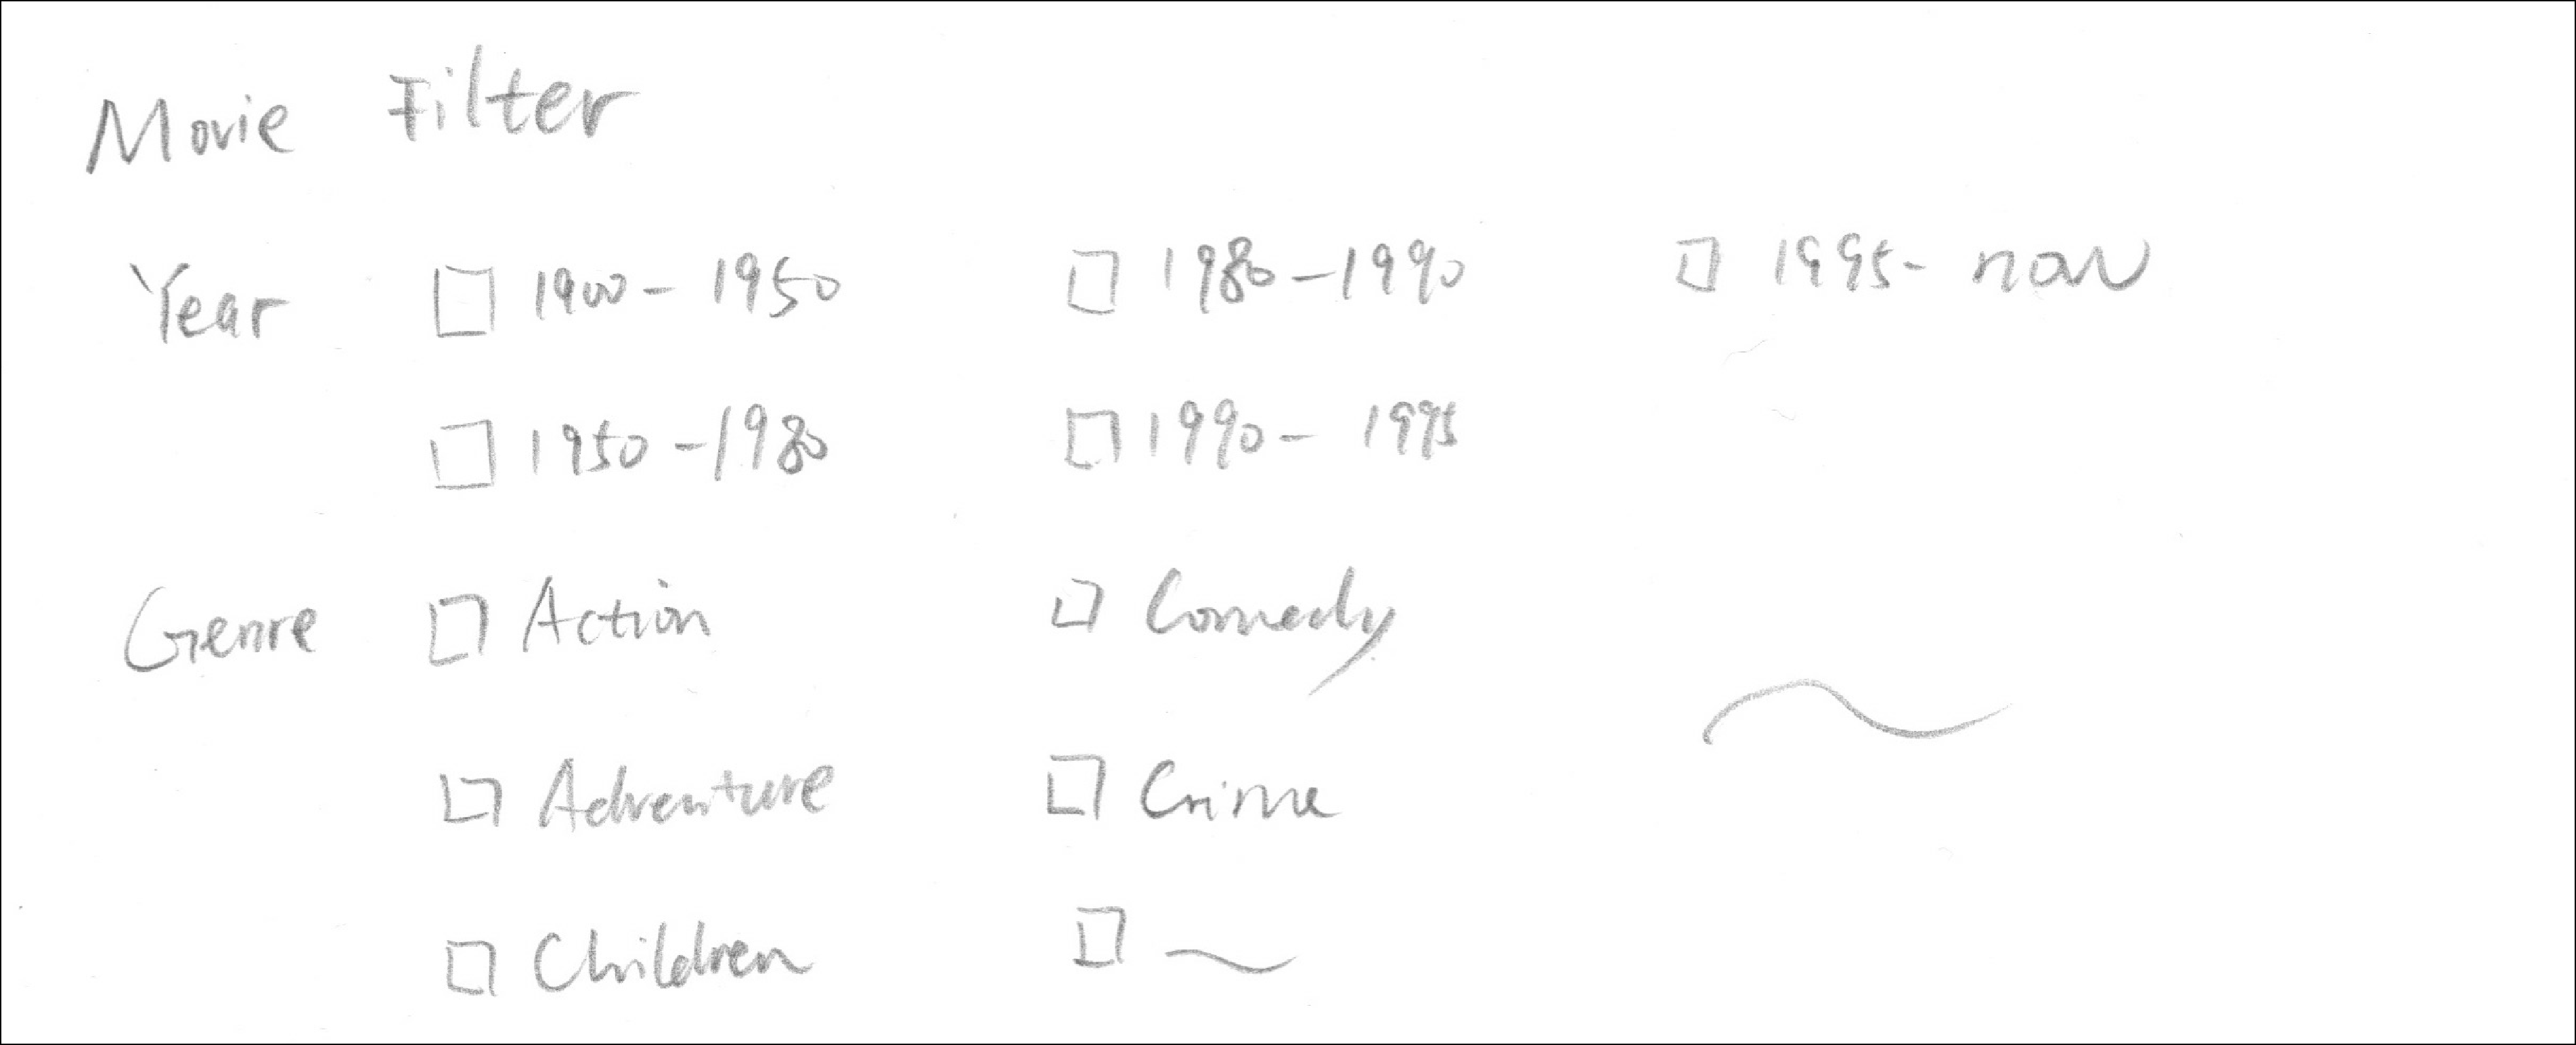
\includegraphics[width=.7\linewidth]{4.pdf}
}
\caption{Filter of movie information}
\label{fig:fig4}
\end{figure}

\begin{figure}[h]
\centering{
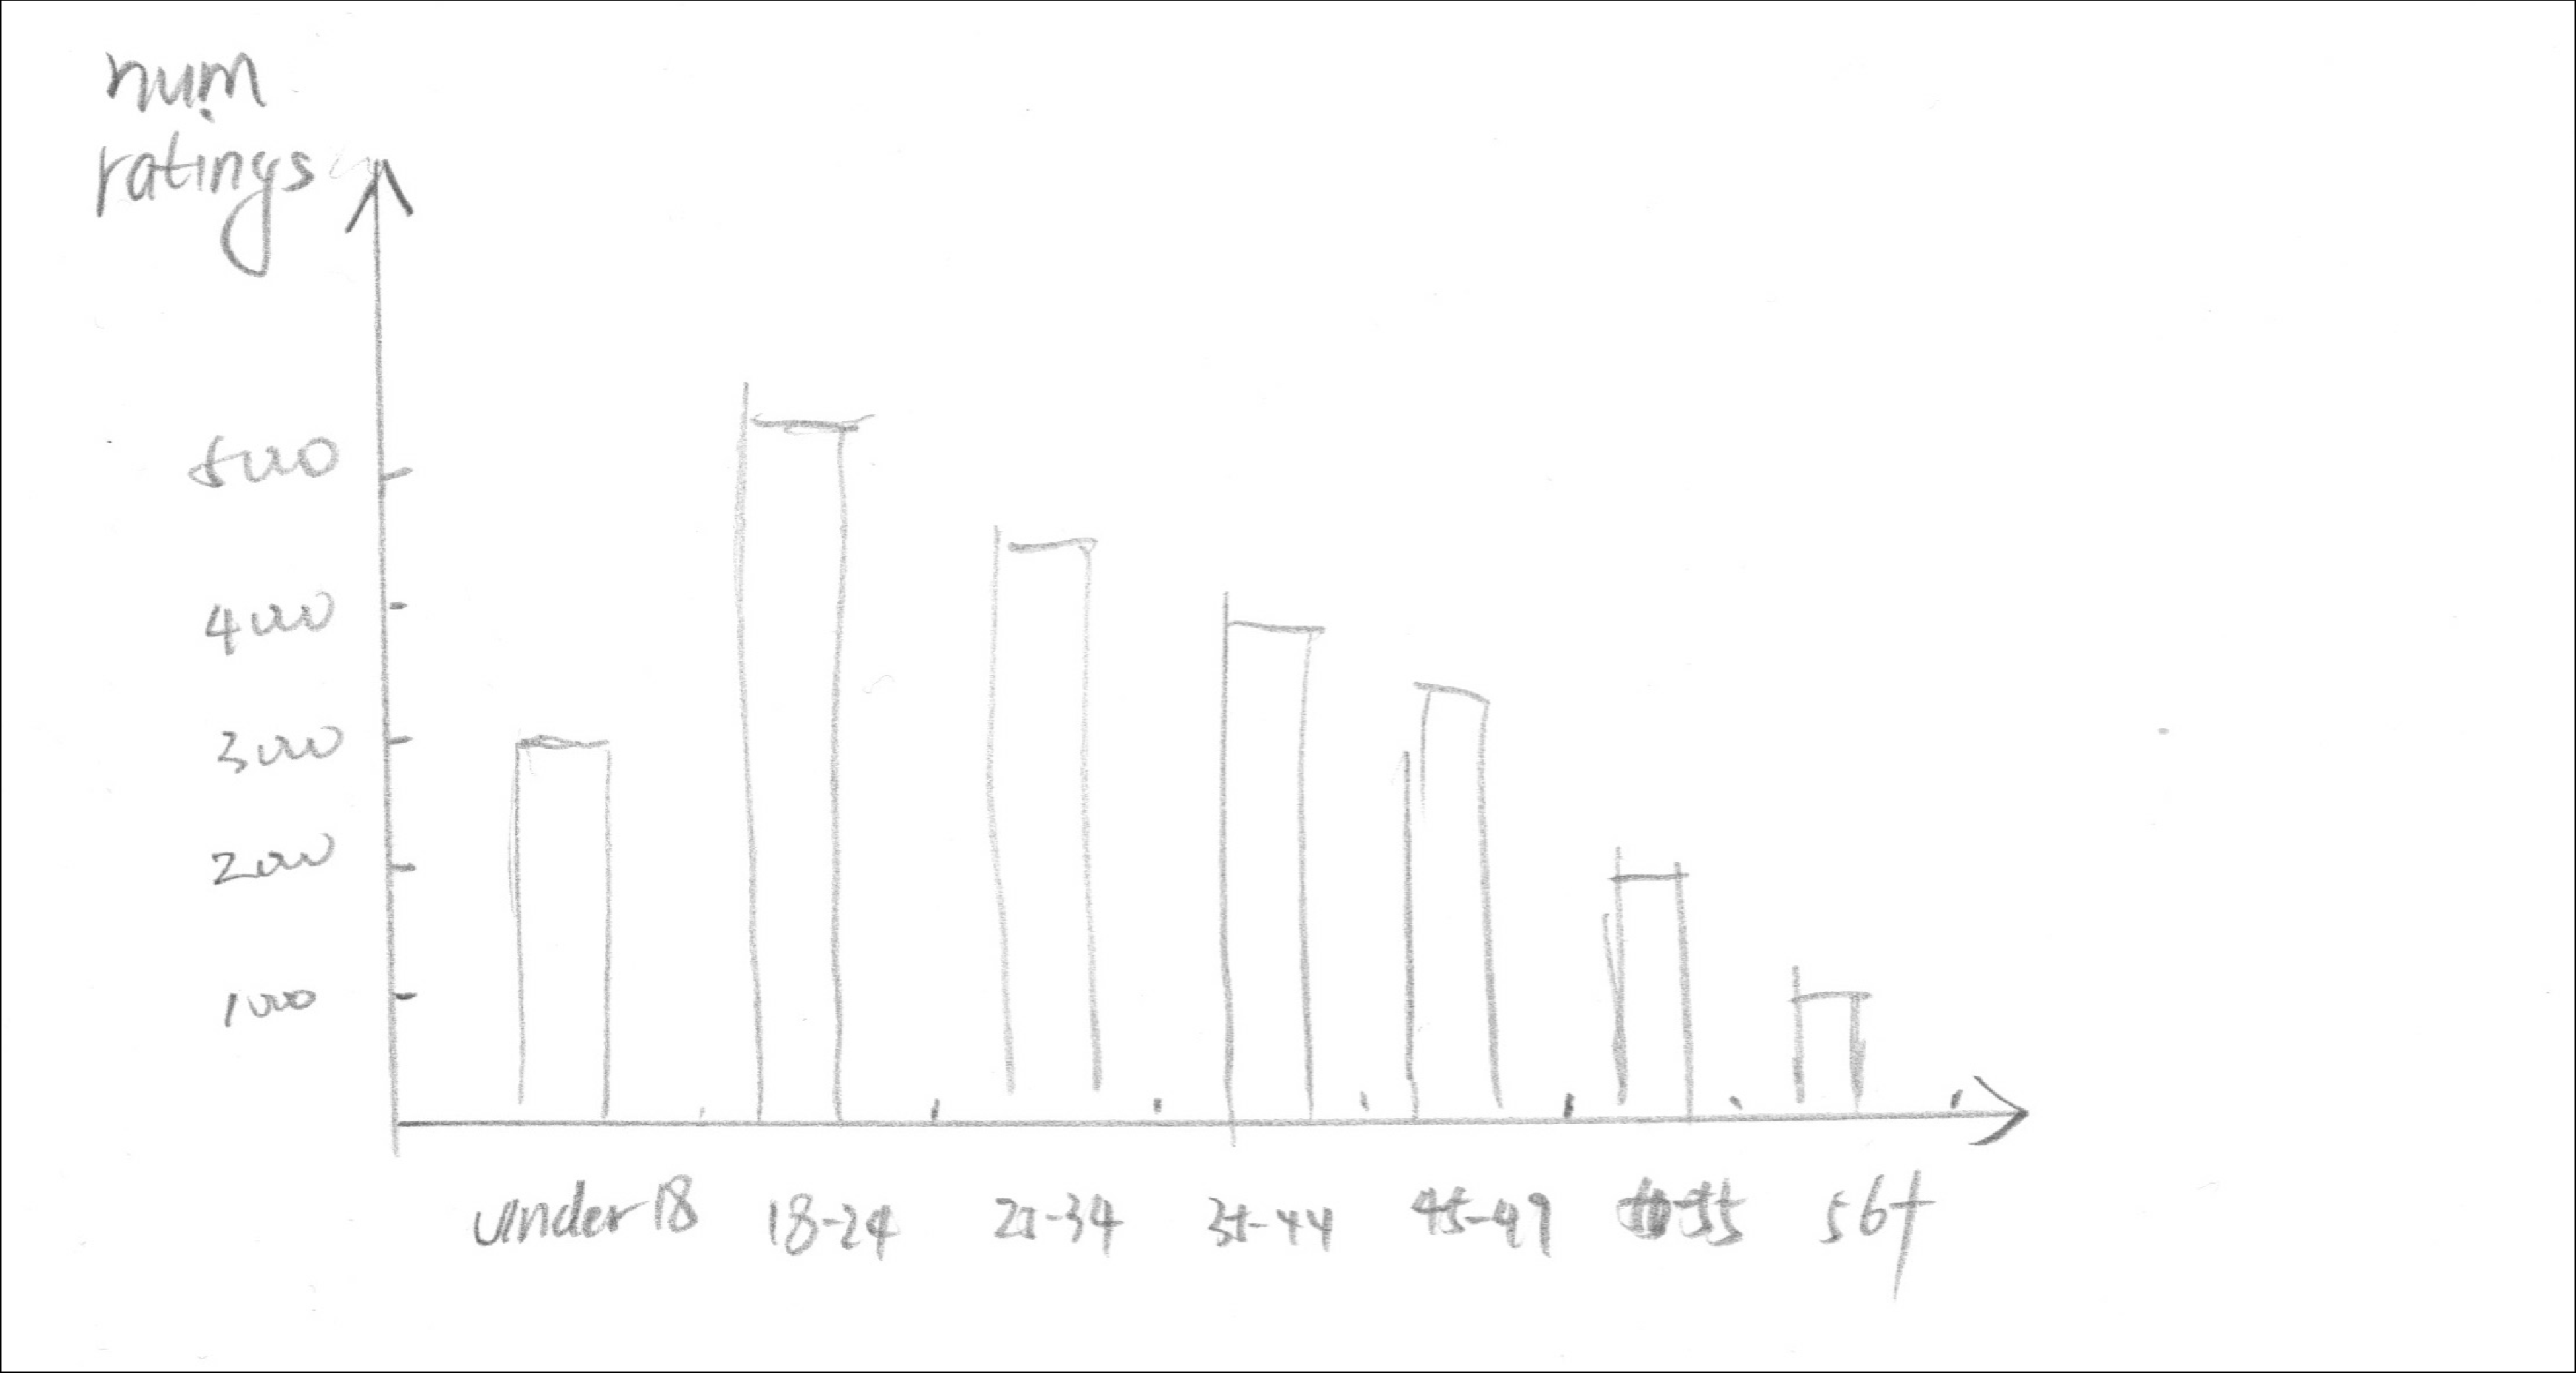
\includegraphics[width=.7\linewidth]{5.pdf}
}
\caption{Number of ratings grouped by ages}
\label{fig:fig5}
\end{figure}

\begin{figure}[h]
\centering{
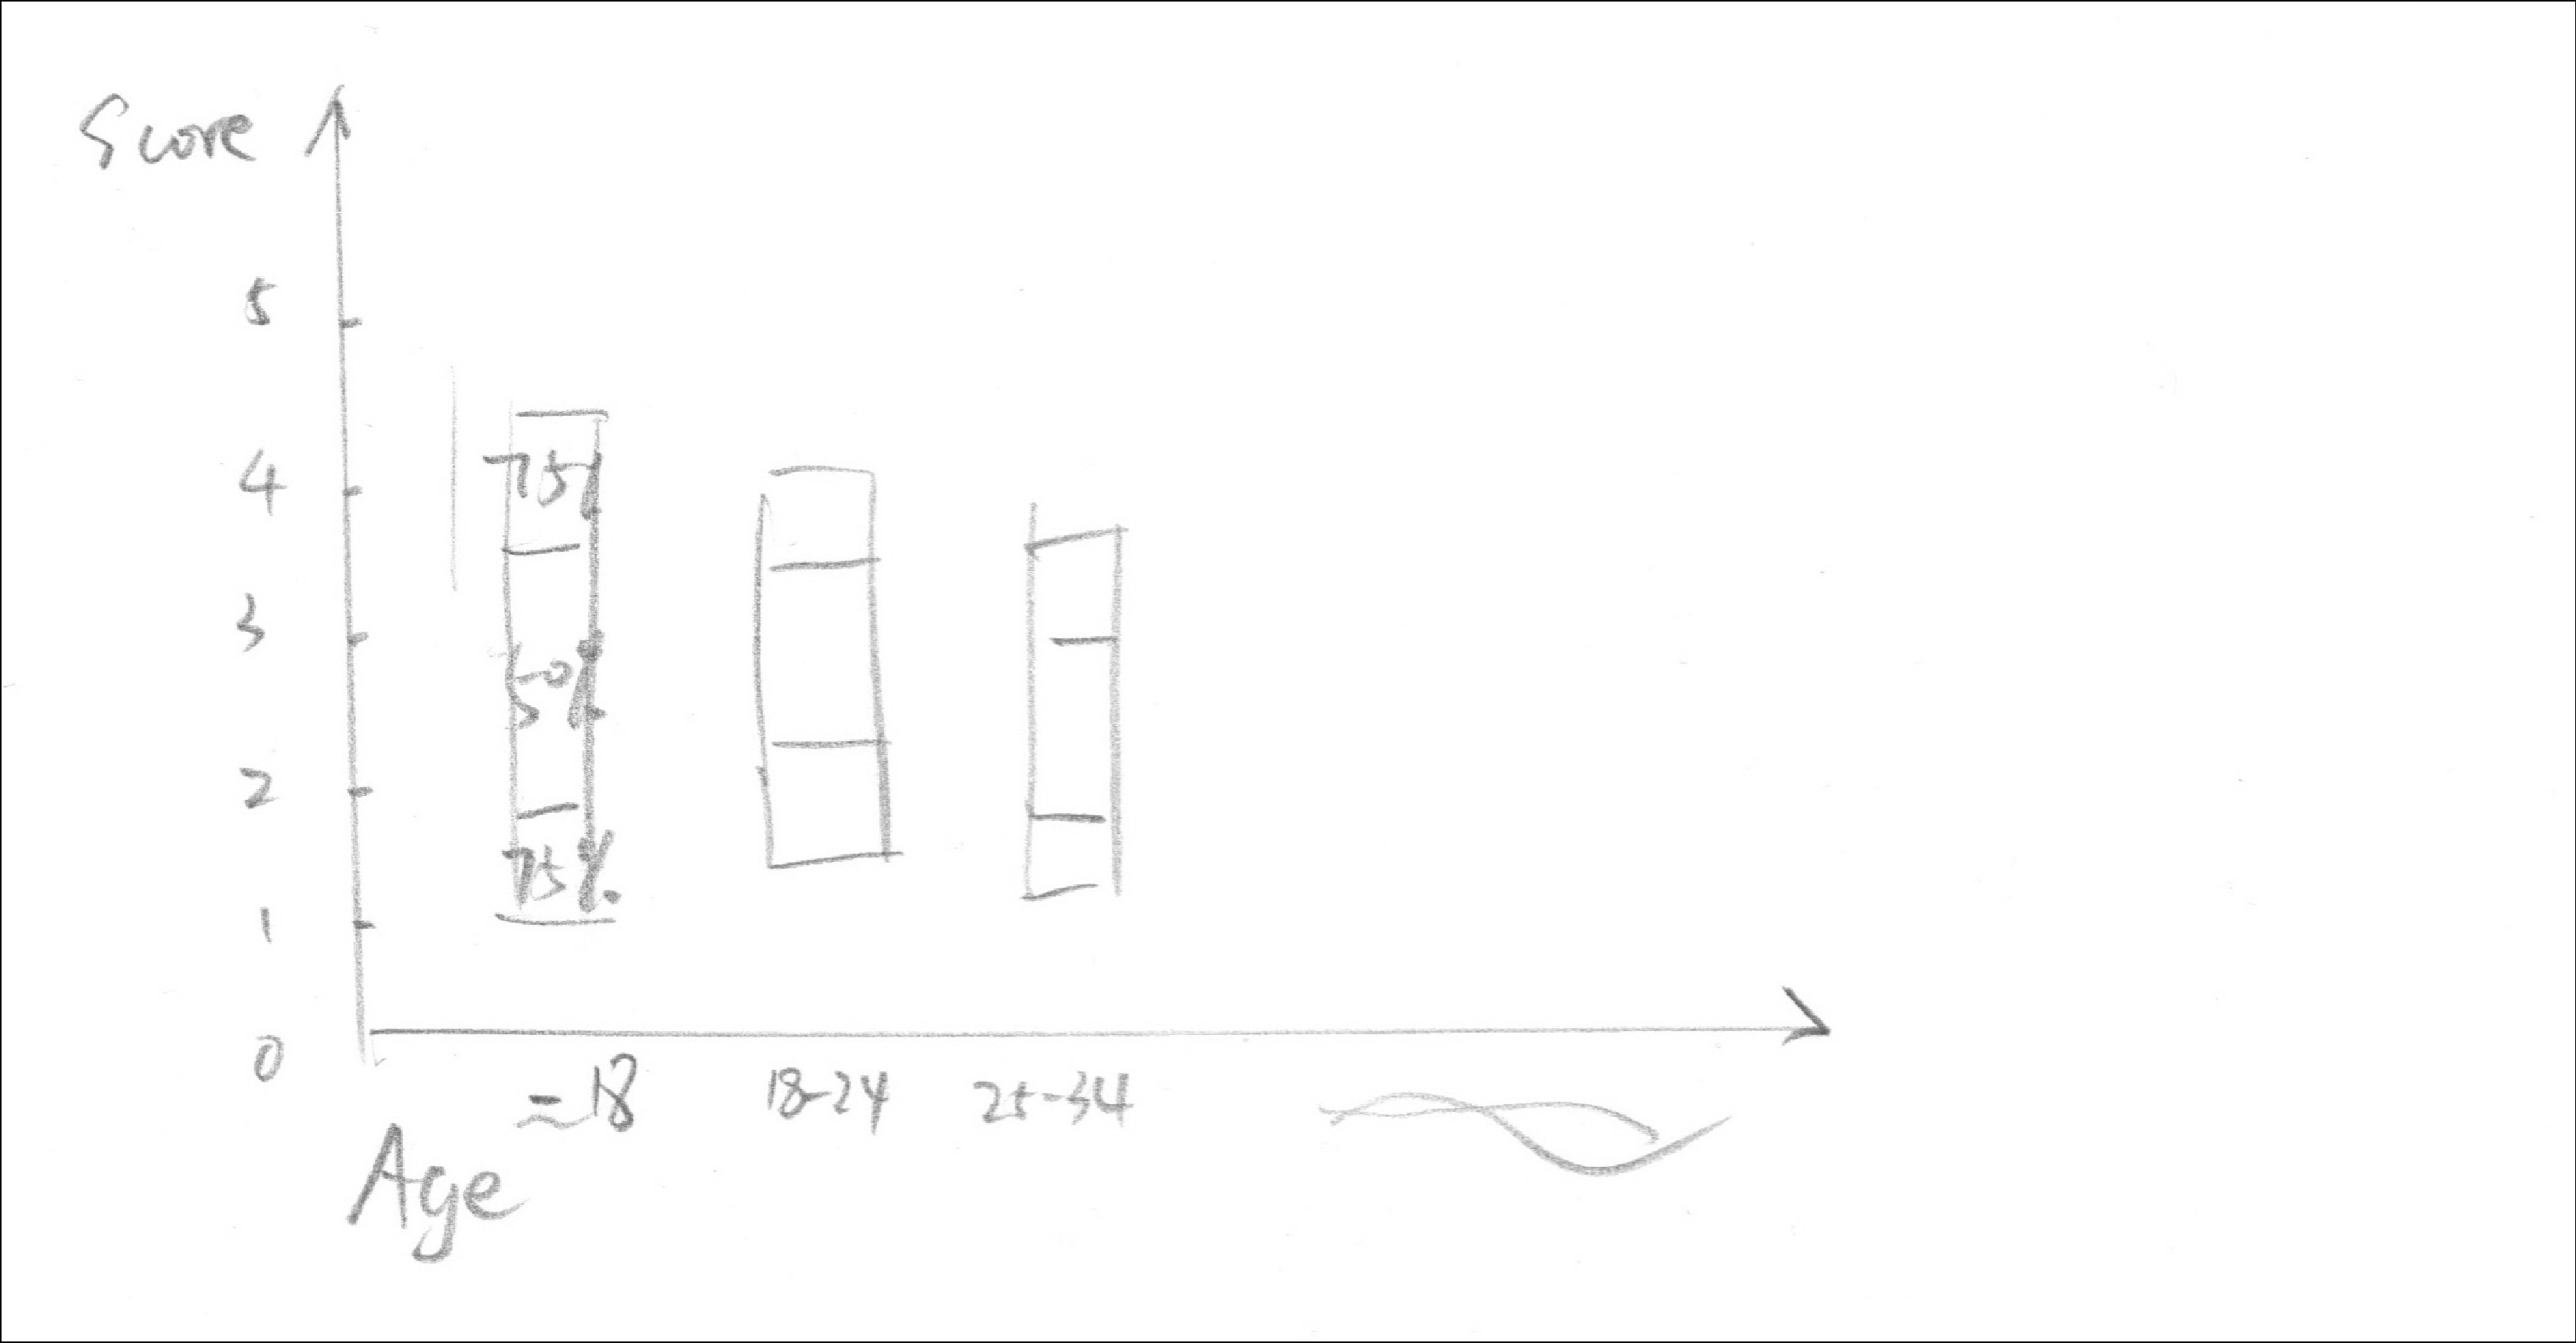
\includegraphics[width=.7\linewidth]{6.pdf}
}
\caption{Distributions of ratings grouped by ages}
\label{fig:fig6}
\end{figure}

\begin{figure}[h]
\centering{
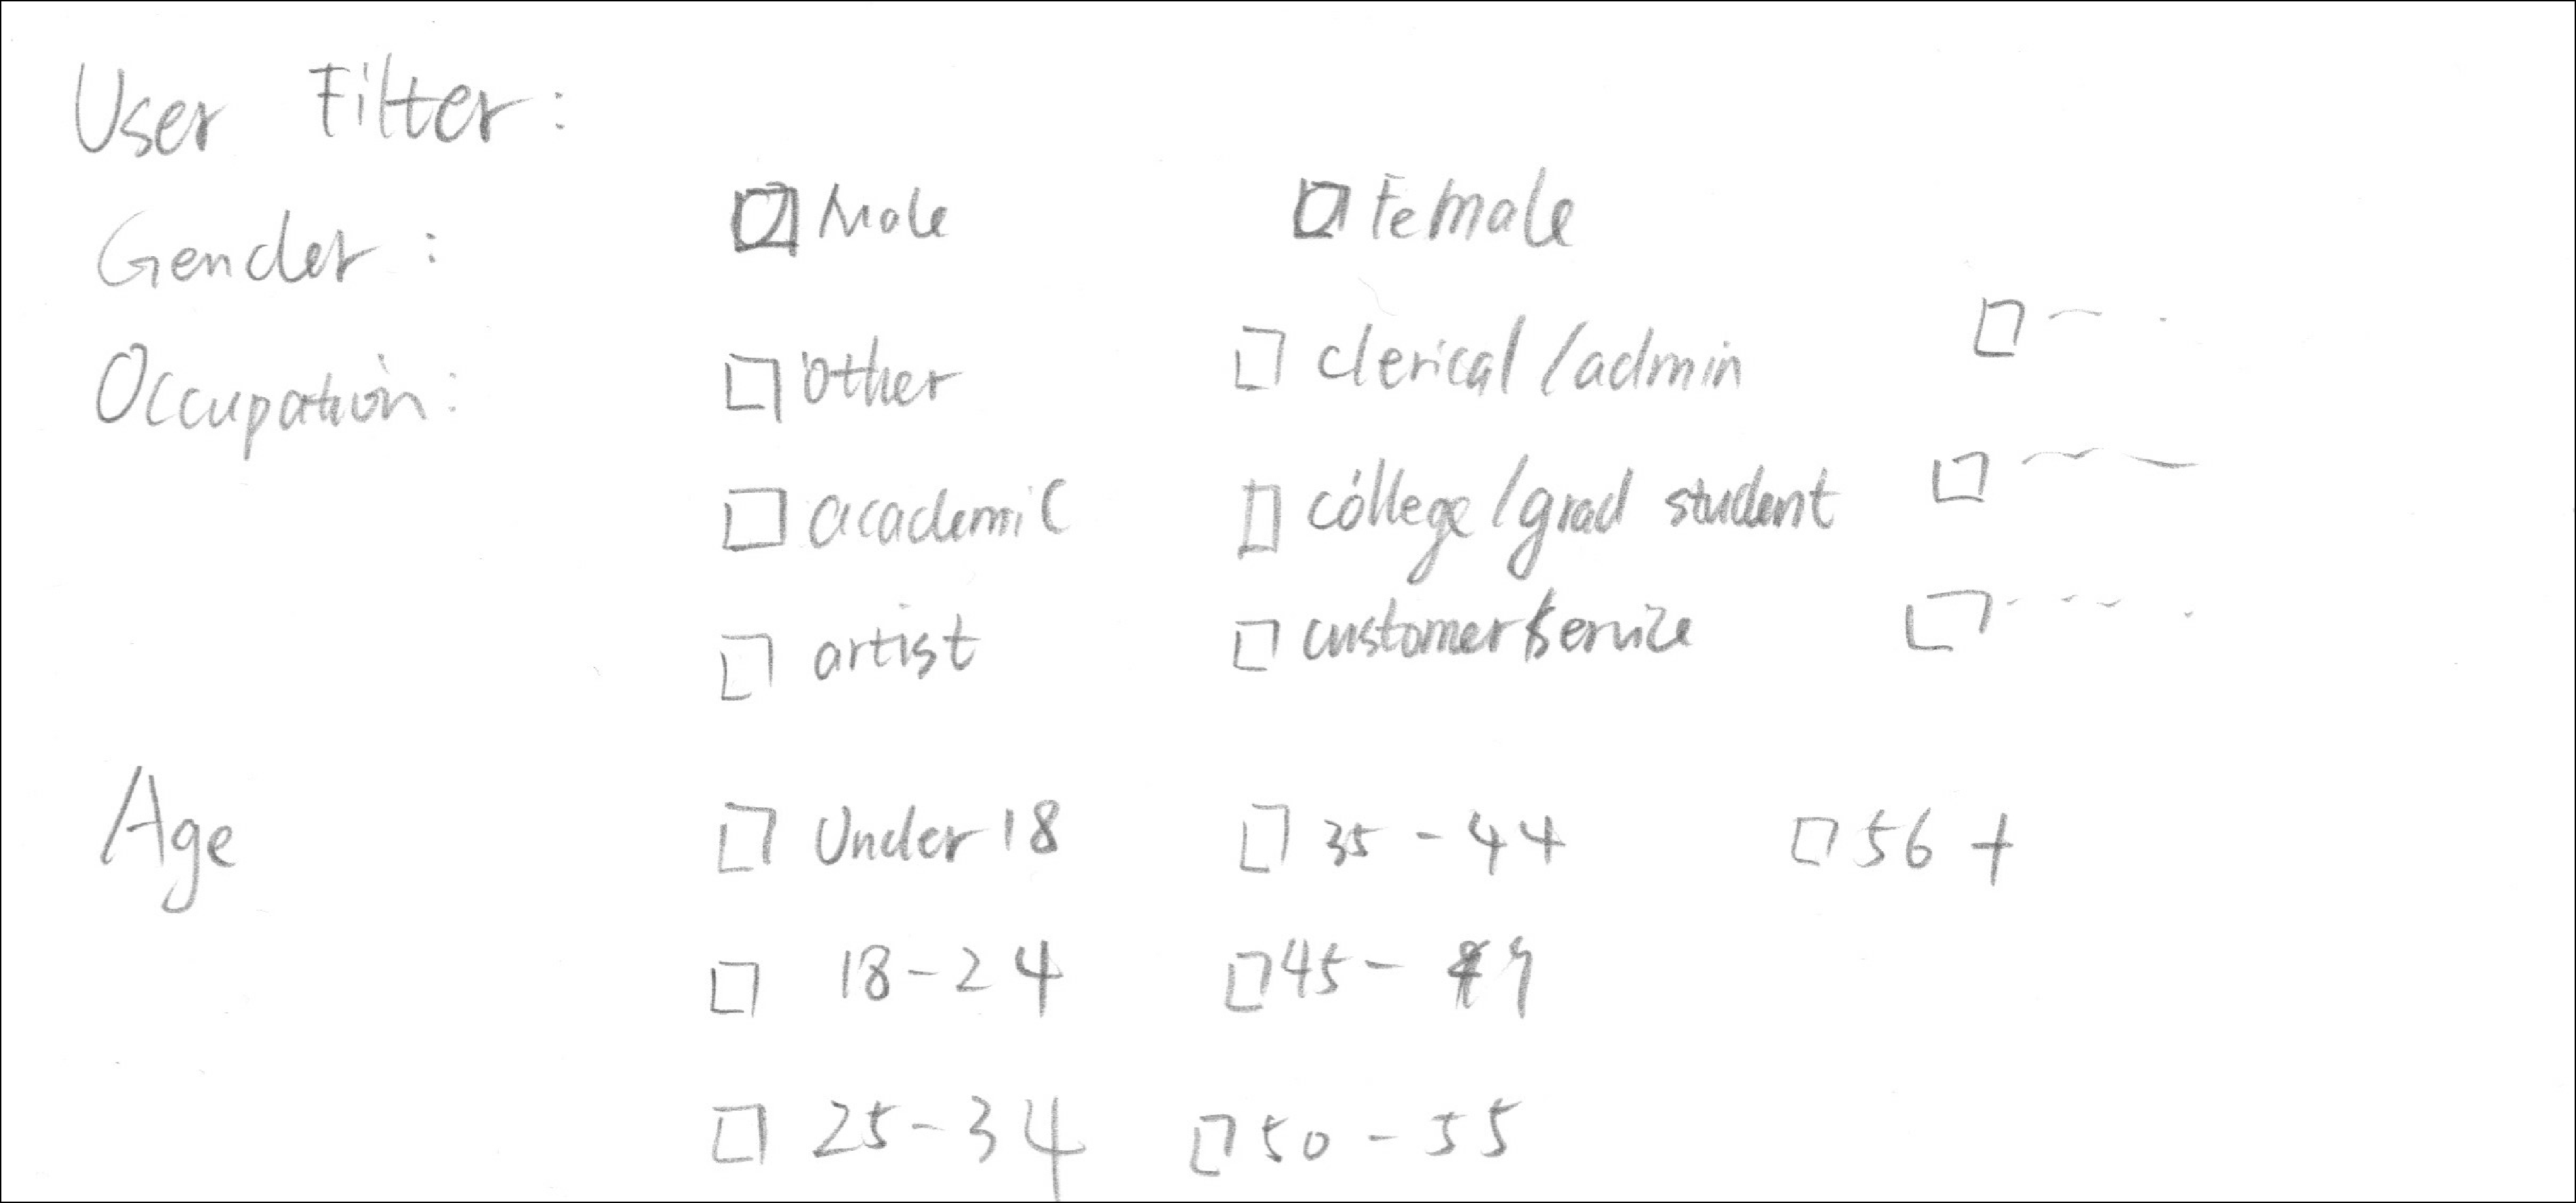
\includegraphics[width=.7\linewidth]{7.pdf}
}
\caption{Filter of user information}
\label{fig:fig7}
\end{figure}

\begin{figure}[h]
\centering{
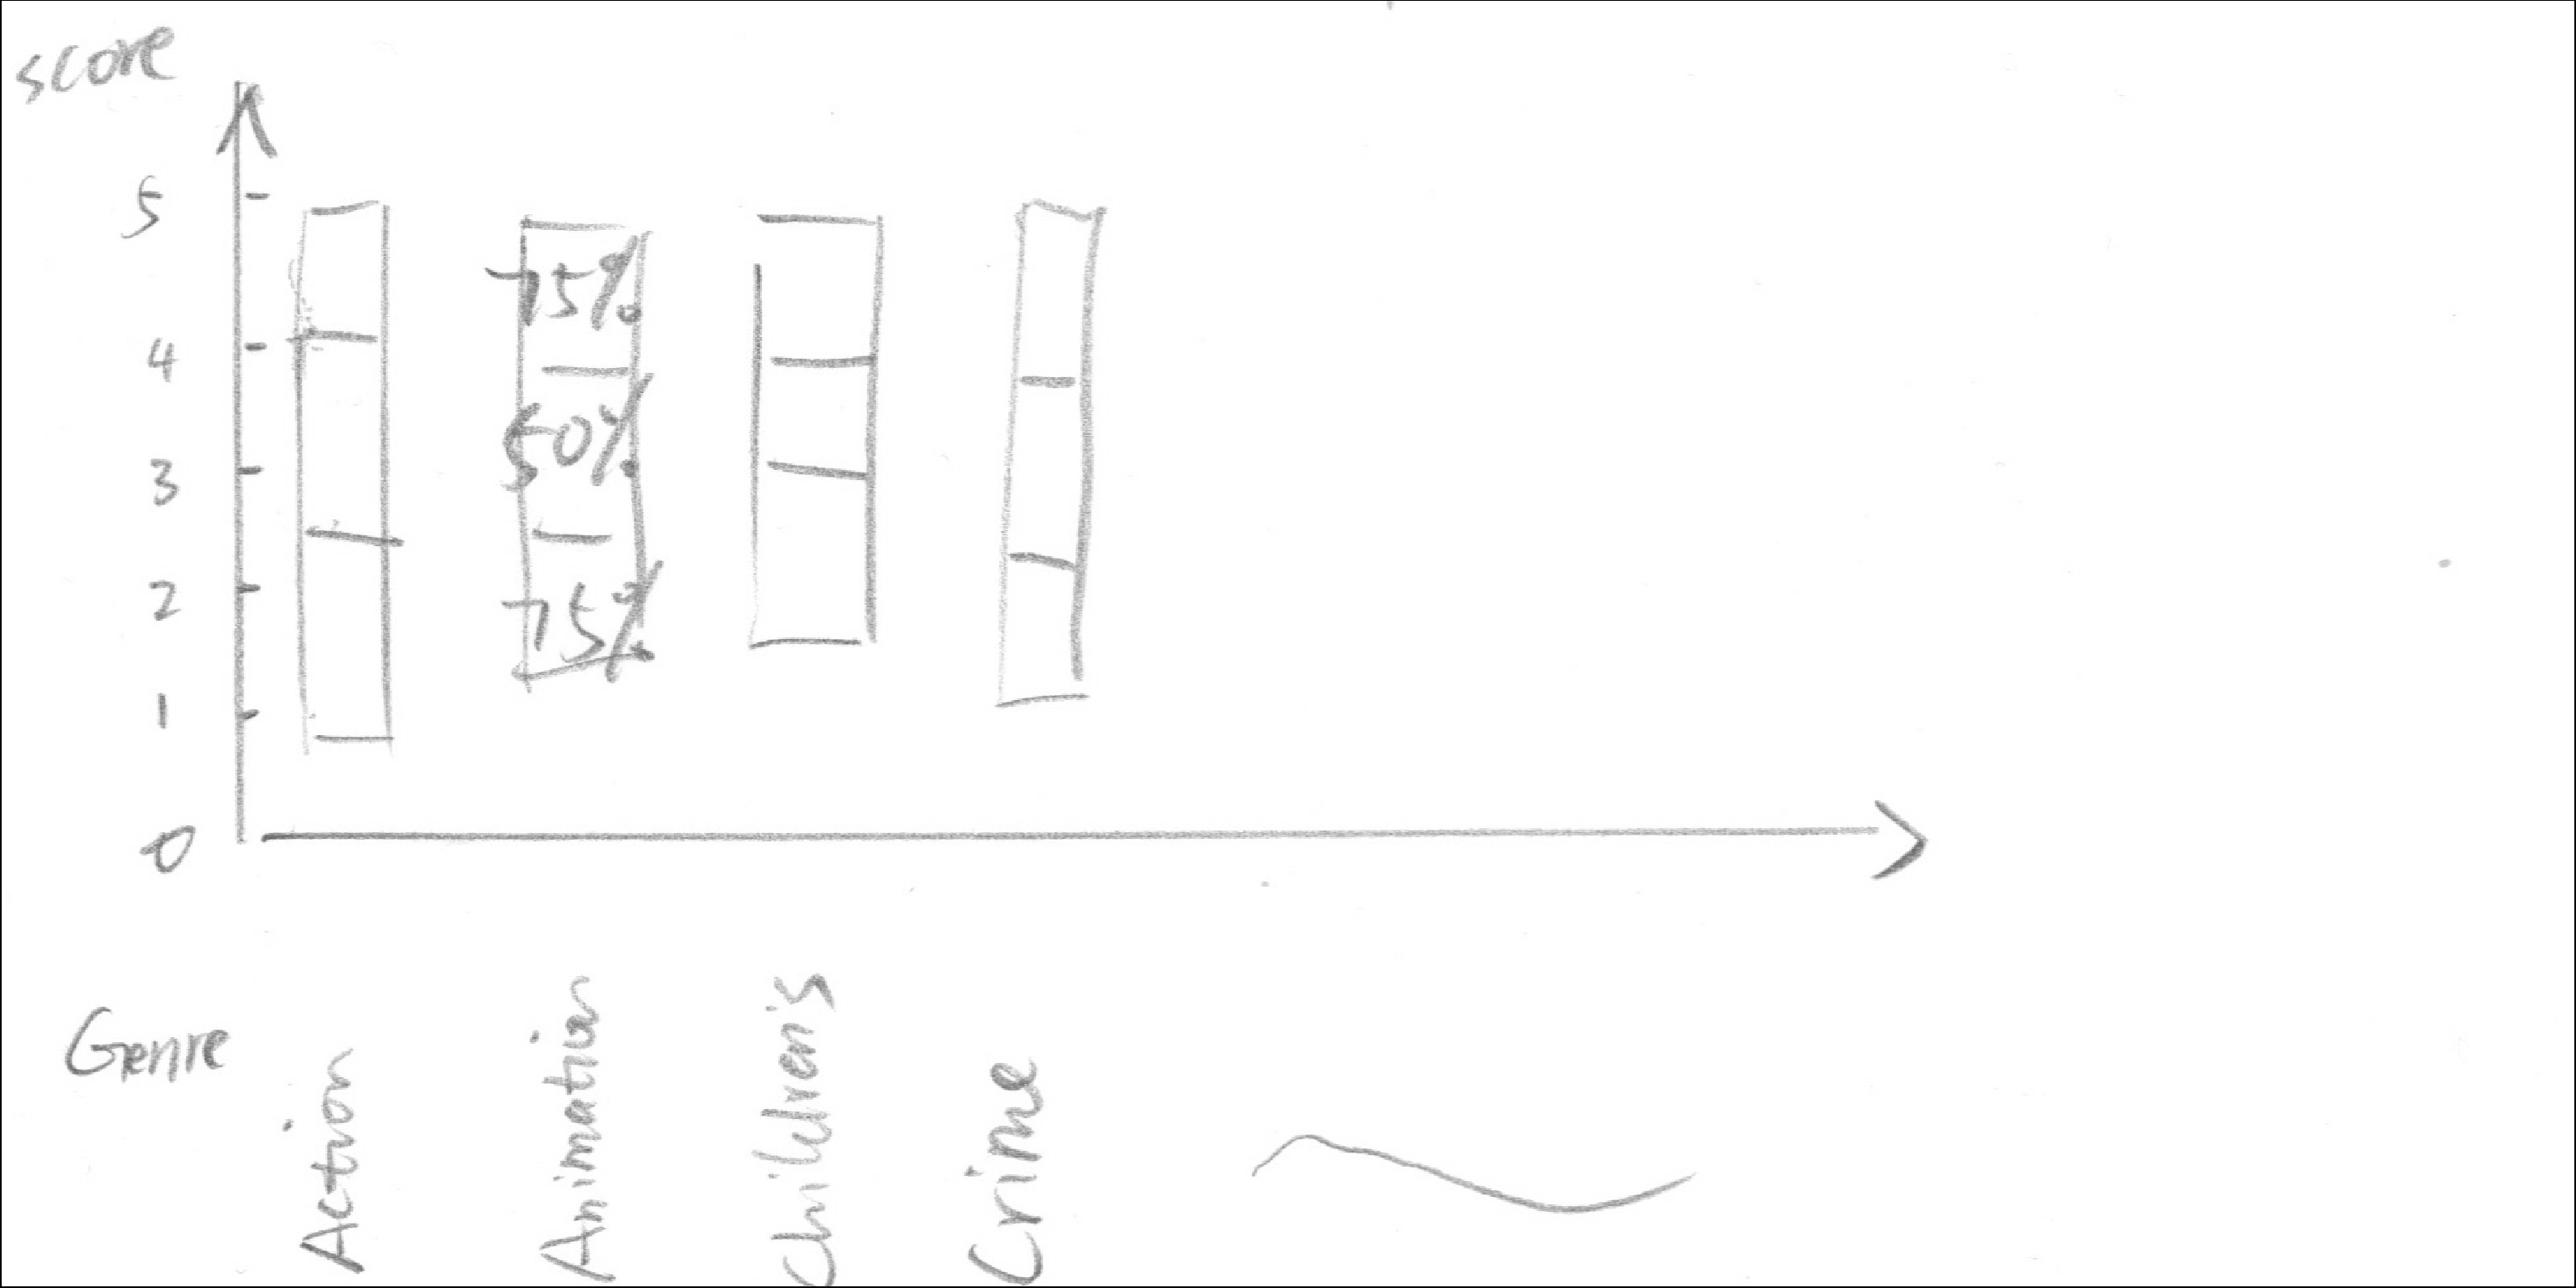
\includegraphics[width=.7\linewidth]{8.pdf}
}
\caption{Distributions of scores grouped by genres}
\label{fig:fig8}
\end{figure}

\begin{figure}[h]
\centering{
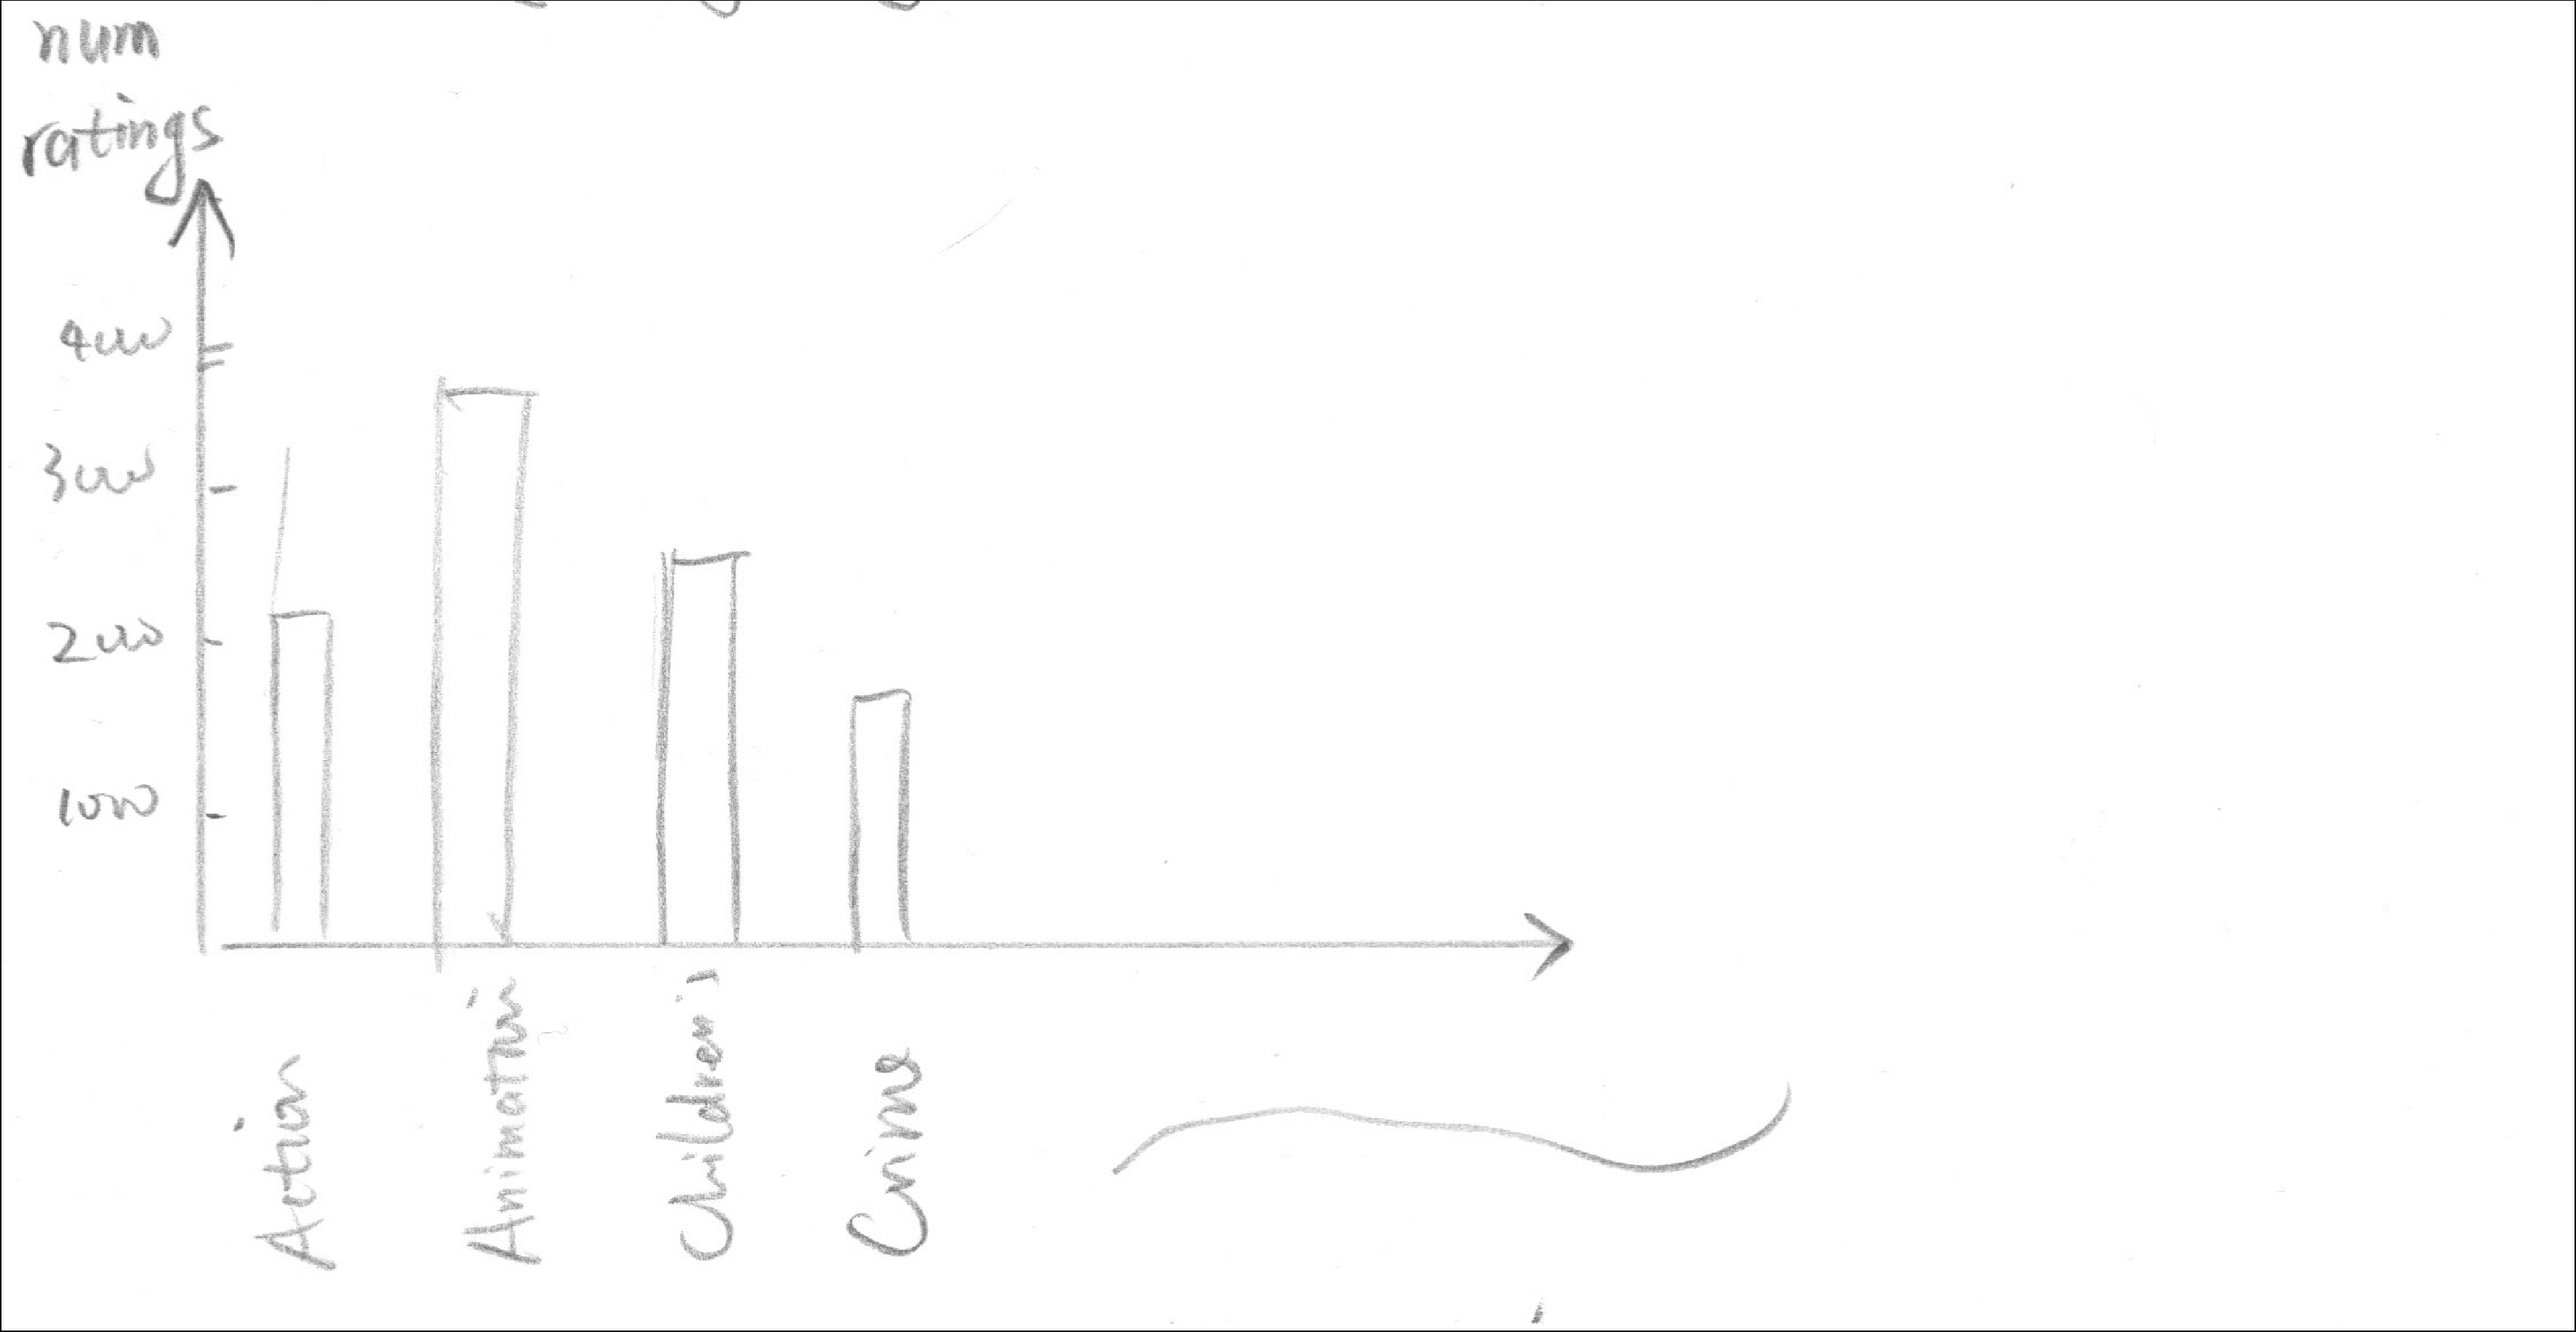
\includegraphics[width=.7\linewidth]{9.pdf}
}
\caption{Number of ratings grouped by genres}
\label{fig:fig9}
\end{figure}

\begin{figure}[h]
\centering{
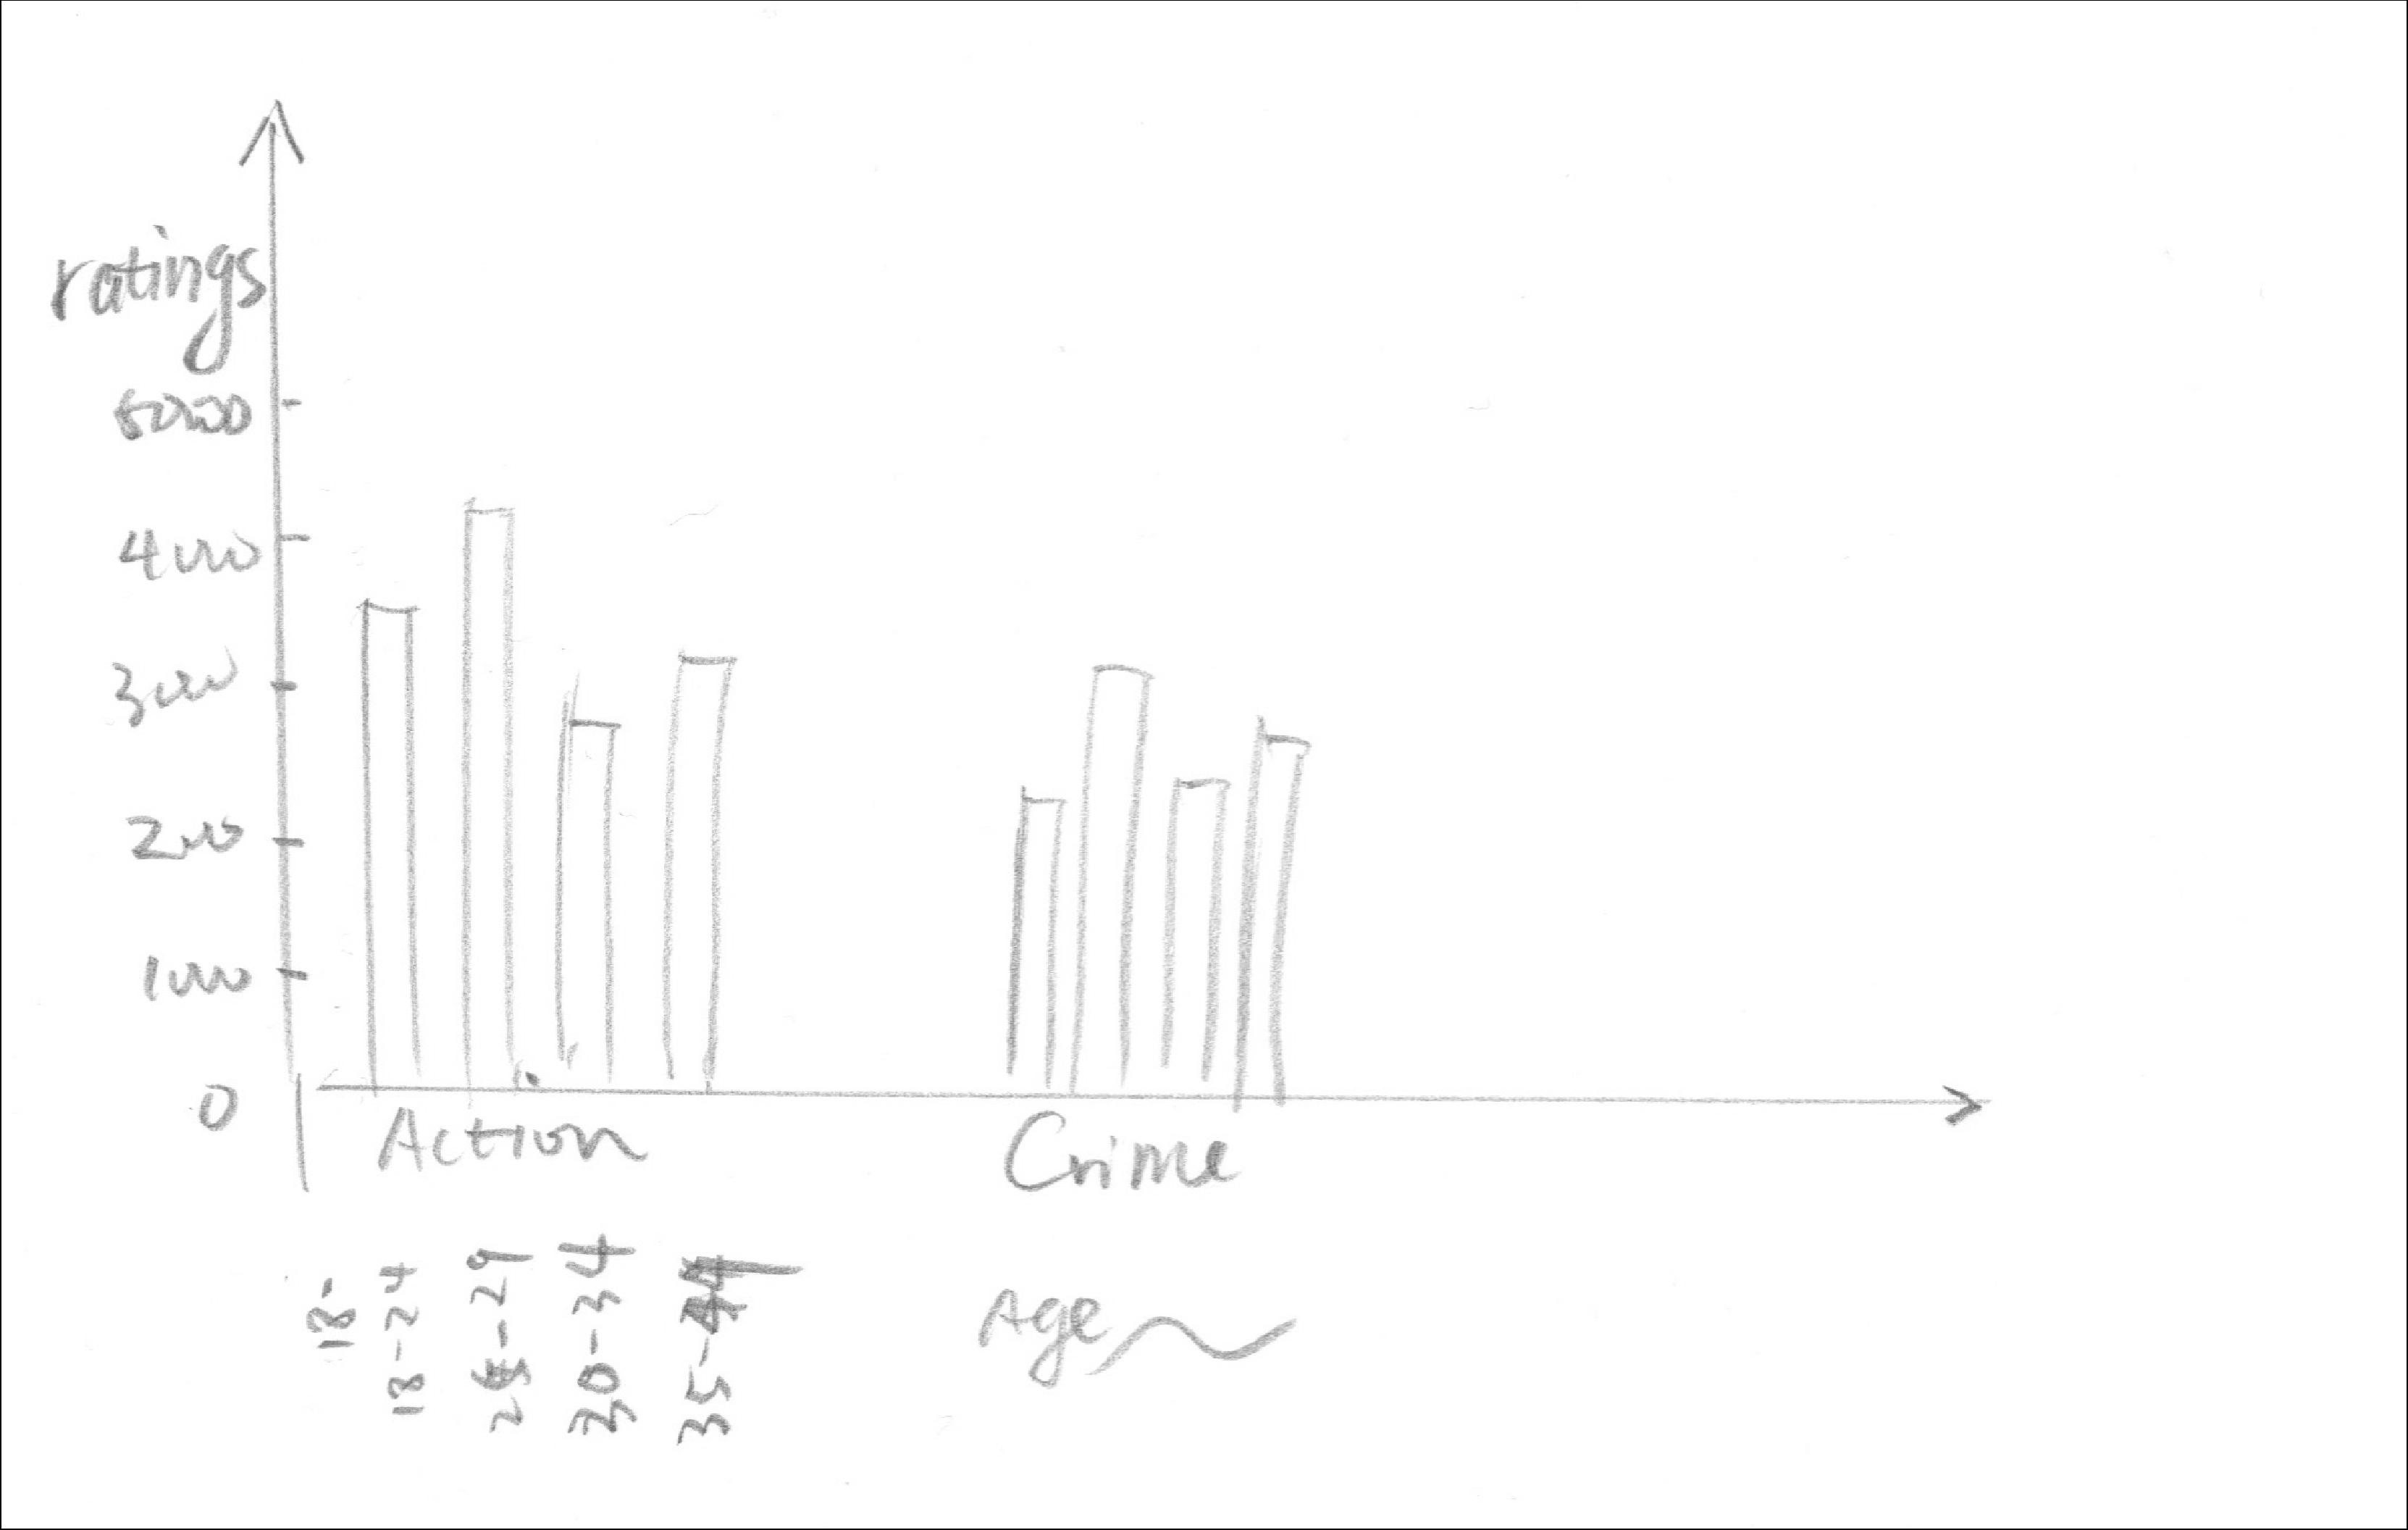
\includegraphics[width=.7\linewidth]{10.pdf}
}
\caption{Number of ratings grouped by genres and subdivided by ages}
\label{fig:fig10}
\end{figure}

\begin{figure}[h]
\centering{
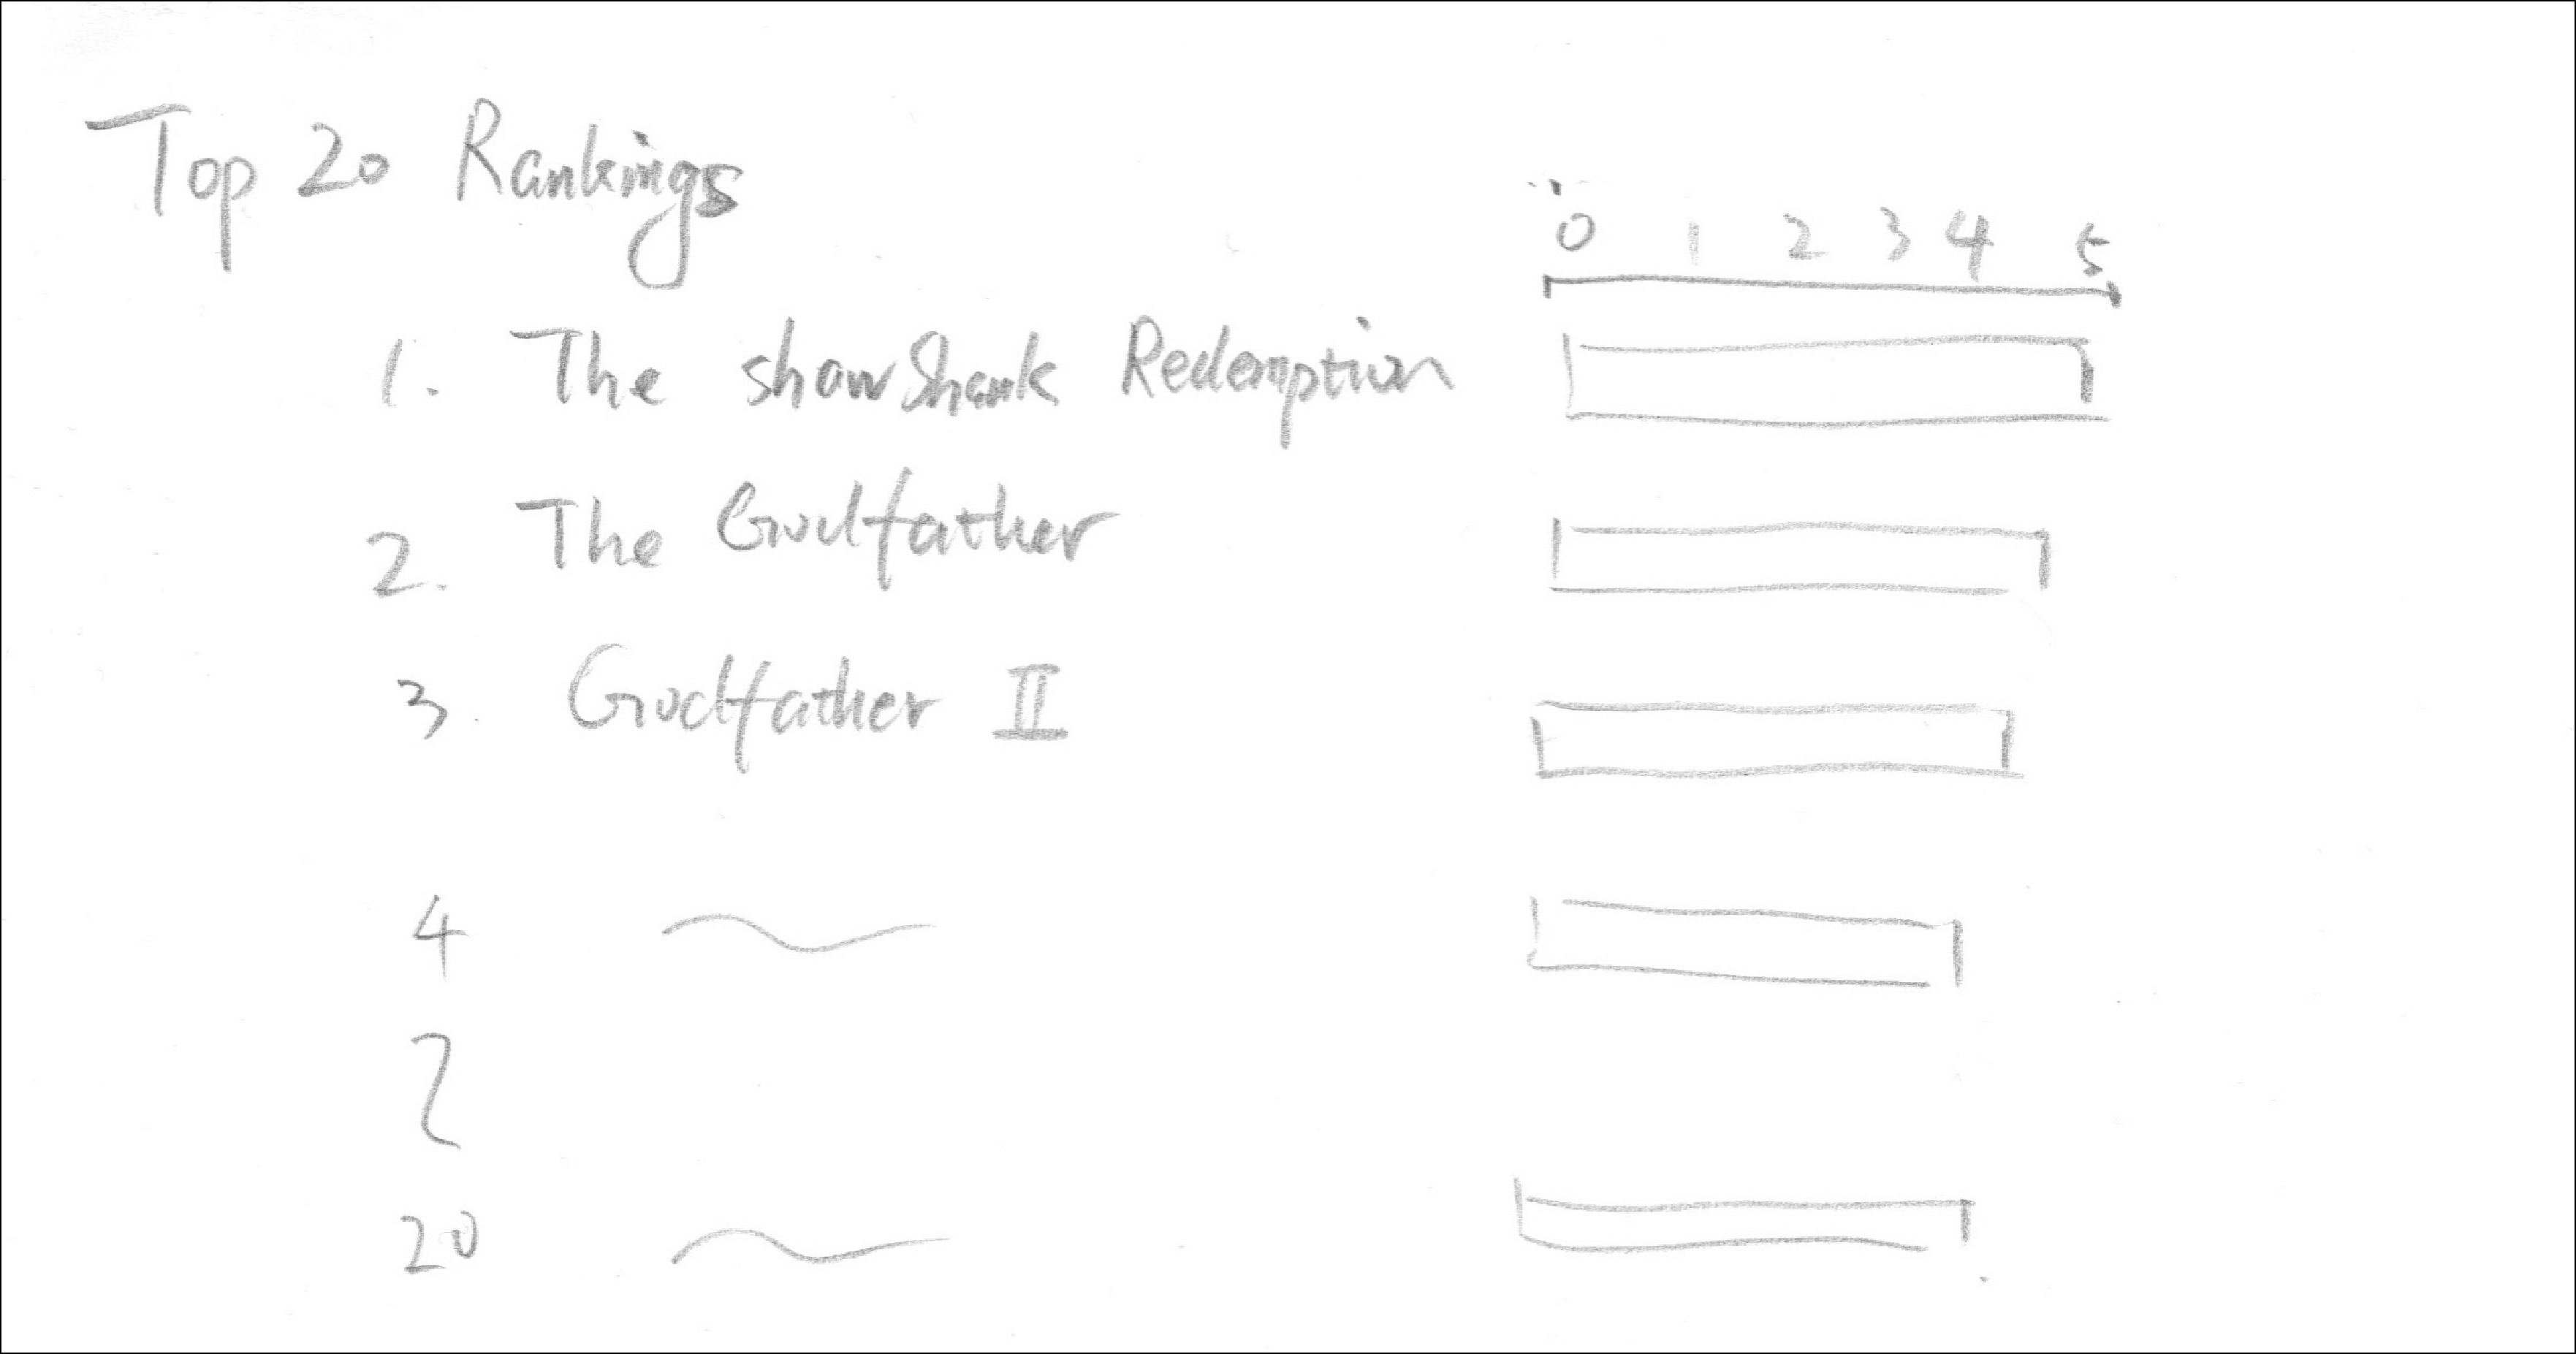
\includegraphics[width=.7\linewidth]{11.pdf}
}
\caption{Rankings of movie scores}
\label{fig:fig11}
\end{figure}

\begin{figure}[h]
\centering{
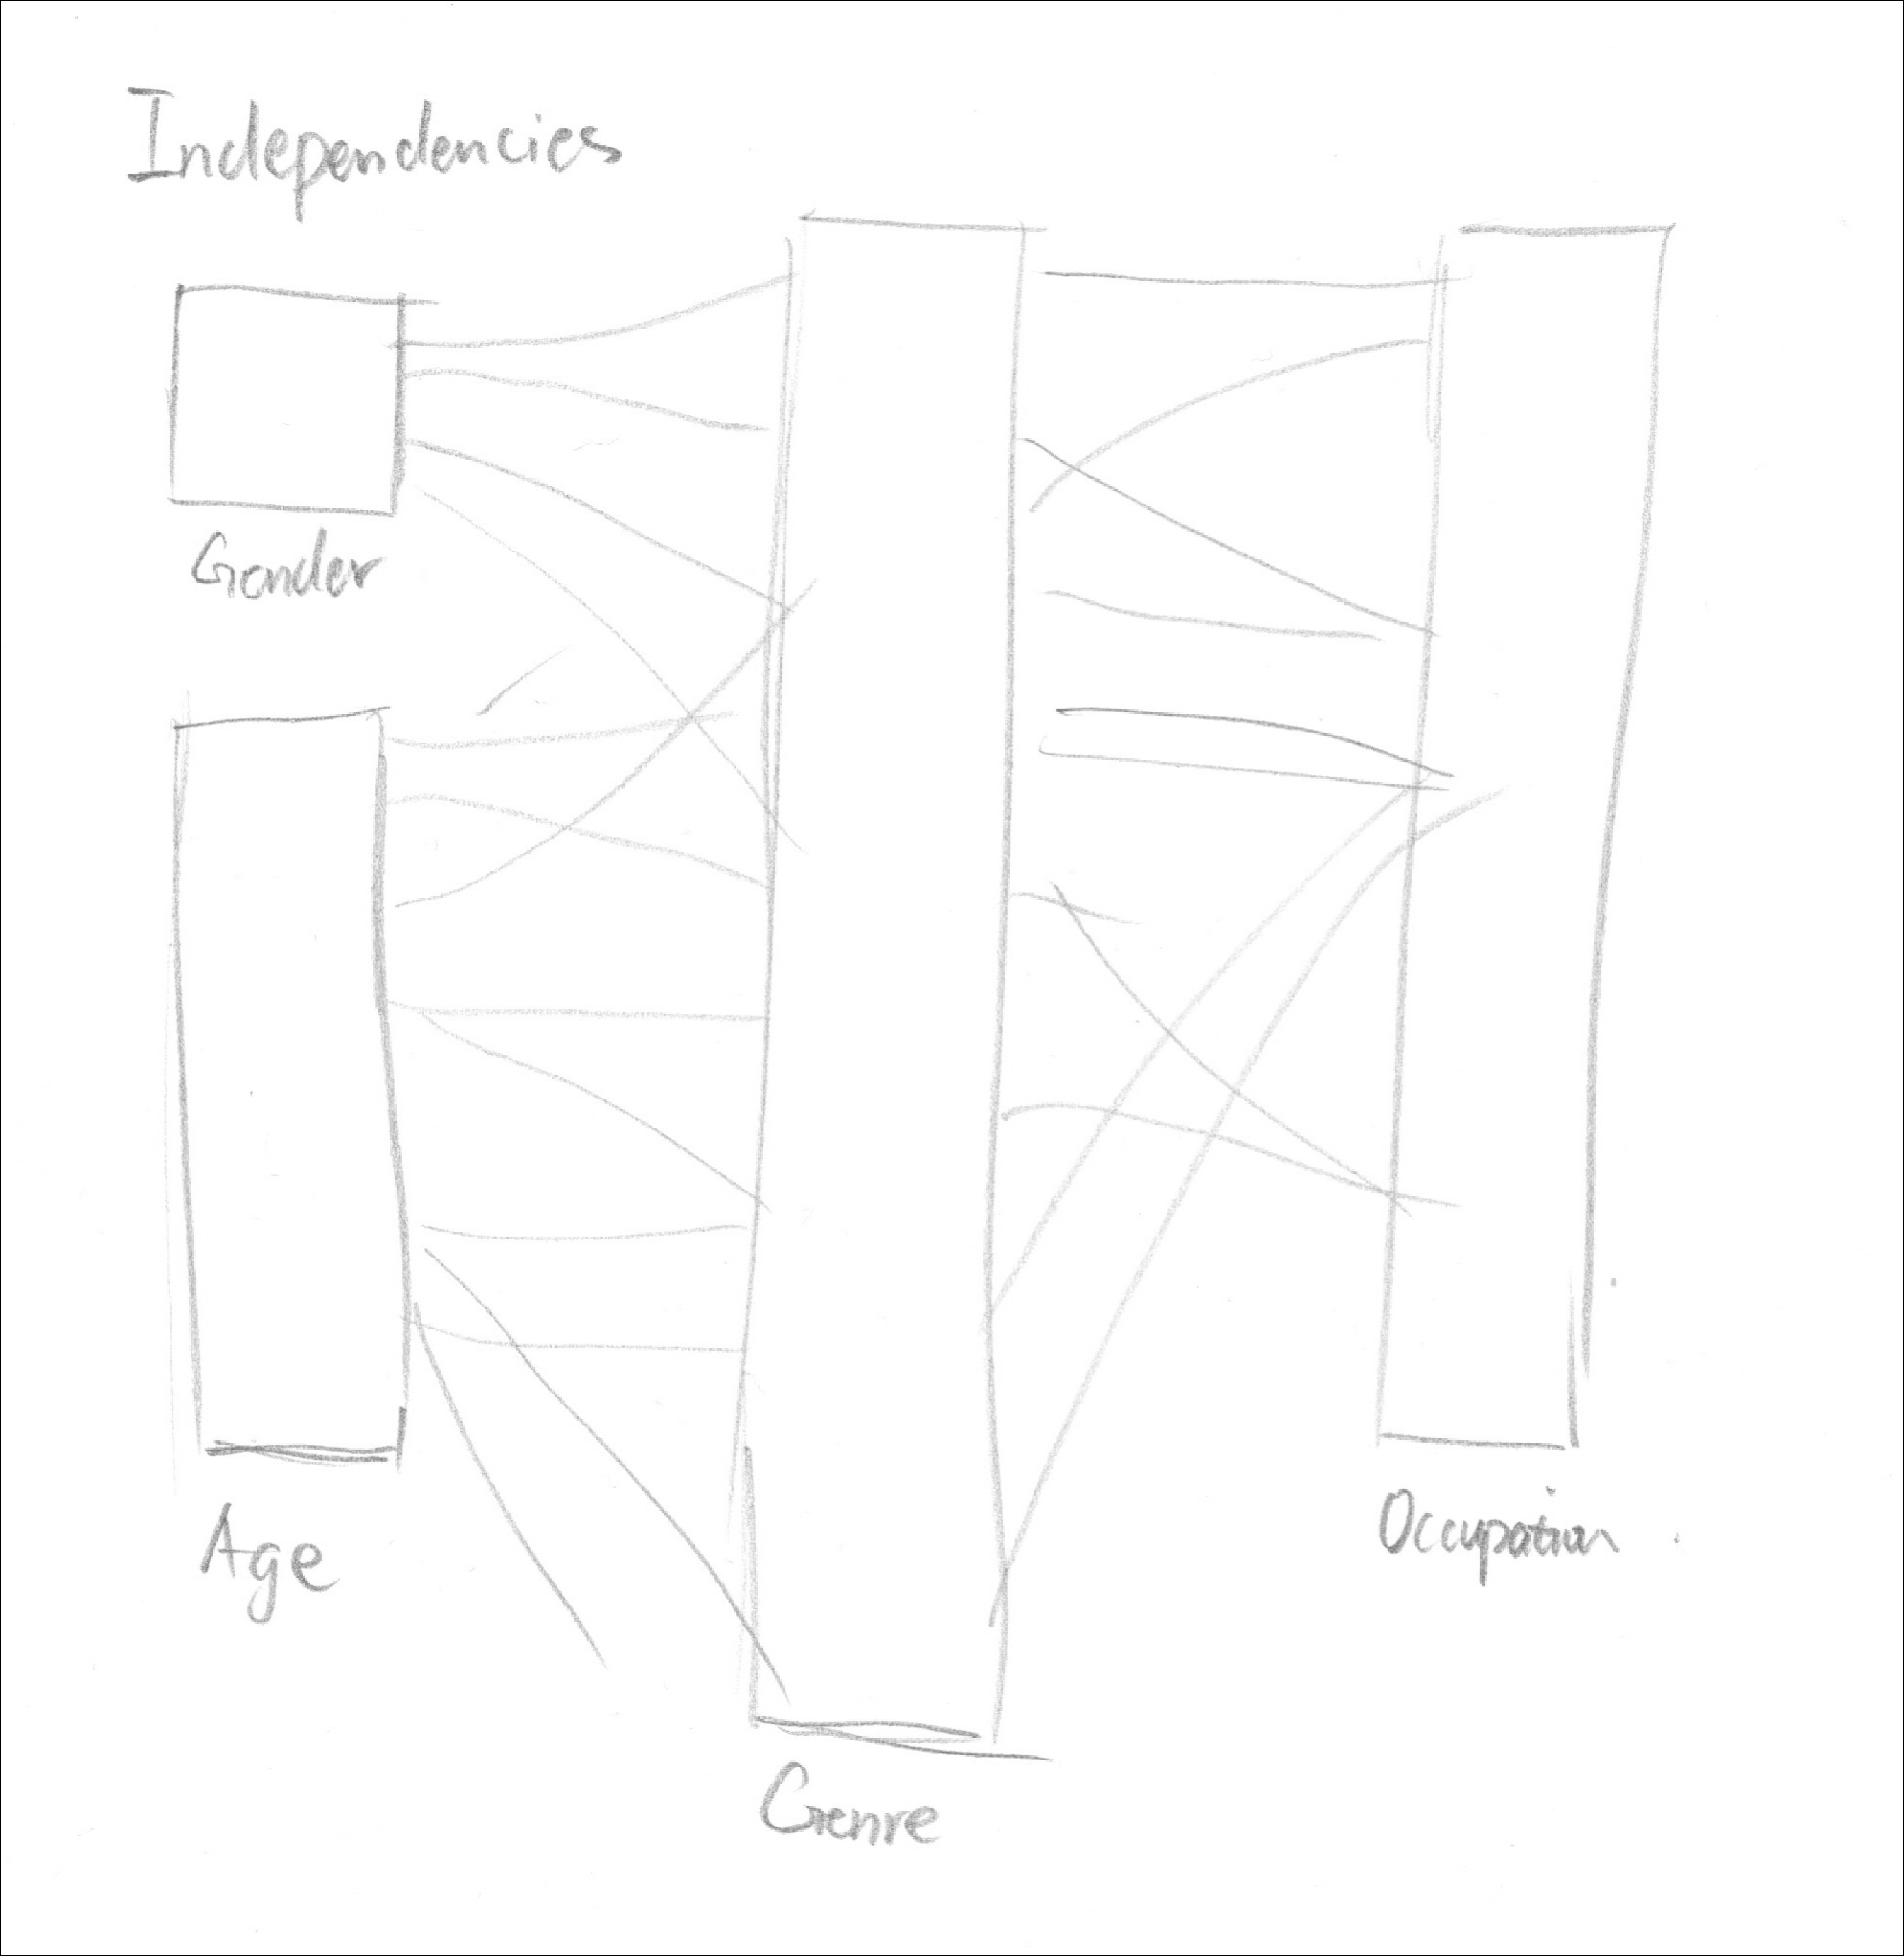
\includegraphics[width=.7\linewidth]{12.pdf}
}
\caption{Dependencies of users and movies}
\label{fig:fig12}
\end{figure}

\subsubsection{Project Peer Feedback}

\begin{itemize}
\item[1)] If the user does not choose some suitable filter options, presenting all the things in the web page may need a considerable cost, since we have a relatively large data set.
\item[2)] They suggest that we may need to add more interactive visualization designs.
\item[3)] Since we have Zip Code information of each person, we can find the corresponding geo-location information. Thus they suggest that we can try visualizing the ratings related with the corresponding locations in the map.
\end{itemize}

\subsection{Our Design in Final Submission}

TBD

\section{Implementation}

\subsection{Our Implementation in Milestone}

\subsubsection{Data Preprocessing}

We simply transformed the original data into the format that can be easily processed. Then we imported the transformed data into MySQL. We used three tables to present the transformed data. The SQL statement ``Create table if not exists Movie( MovieID int, Title varchar(100), Genres varchar(50) )'' can create Movie table. The SQL statement ``Create table if not exists User( UserID int, Gender int, Age int, Occupation int, ZipCode varchar(15) )'' can create User table. The SQL statement ``Create table if not exists Movie( MovieID int, Title varchar(100), Genres varchar(50) )'' can create Movie table. The SQL statement ``Create table if not exists Rating( UserID int, MovieID int, Rating int, Timestamp varchar(15) )'' can create Rating table. After inserting the tuples into the tables in the database, we can easily gain some statistics by performing the corresponding aggregate queries.

\subsubsection{Basic Visualization Design}

Build the basic visual structure/layout using JavaScript.

\subsection{Our Implementation in Final Submission}

TBD

\section{Evaluation}

What do we learn about the data by using our visualizations?

TBD

How do we answer our questions?

TBD

How well does our visualization work, and how could we further improve it?

TBD

\pagebreak
\restoregeometry
\begin{thebibliography}{}
\bibitem{WWW2001}
B. Sarwar, G. Karypis, J. Konstan, and J. Riedl. Item-based collaborative filtering recommendation algorithms. In \textit{WWW}, pages 285-295, 2001.

\bibitem{IEEE2003}
G. Linden, B. Smith, and J. York. Amazon. com recommendations: Item-to-item collaborative filtering. In \textit{Internet Computing, IEEE}, 7(1), pages 76-80, 2003.

\bibitem{IJCAI2013}
D. Jannach. Tutorial: Recommender systems. In \textit{IJCAI}, 2013.

\bibitem{AAAI1998}
C. Basu, H. Hirsh, and W. Cohen. Recommendation as classification: Using social and content-based information in recommendation. In \textit{AAAI/IAAI}, pages 714-720, 1998.

\bibitem{DL2000}
R. Mooney and L. Roy. Content-based book recommending using learning for text categorization. In \textit{Proceedings of the fifth ACM conference on Digital libraries}, pages 195-204, 2000.

\bibitem{ELIS2000}
R. Burke. Knowledge-based recommender systems. In \textit{Encyclopedia of library and information systems} 69, Supplement 32, pages 175-186, 2000.

\bibitem{WWW2008}
B. Sigurbj{\"o}rnsson and R. V. Zwol. Flickr tag recommendation based on collective knowledge. In \textit{WWW}, pages 327-336, 2008.

\bibitem{WWW20082}
S. Debnath, N. Ganguly, and P. Mitra. Feature weighting in content based recommendation system using social network analysis. In \textit{WWW}, pages 1041-1042, 2008.

\bibitem{UCS2011}
M. Pham, Y. Cao, and R. Klamma. A clustering approach for collaborative filtering recommendation using social network analysis. In \textit{J. UCS}, 17(4), pages 583-604, 2011.

\bibitem{RS2009}
O. Phelan, K. McCarthy, and B. Smyth. Using twitter to recommend real-time topical news. In \textit{Recommender systems}, pages 385-388, 2009.

\bibitem{IR2011}
O. Phelan, K. McCarthy, M. Bennett, and B. Smyth. Terms of a feather: Content-based news recommendation and discovery using twitter. In \textit{Advances in Information Retrieval}, pages 448-459, Springer Berlin Heidelberg, 2011.
\end{thebibliography}
\end{document}
